\documentclass[french, 10pt]{beamer}
\usetheme{Darmstadt}
\usepackage{csquotes}
\usepackage{graphicx}
\usepackage{algorithm2e}
\usepackage{wrapfig}
\usepackage{ragged2e}
\usepackage{amsmath, amssymb}
\usepackage[french]{babel}
\usepackage{multirow}
\usepackage[many,skins]{tcolorbox}

\usepackage[numbers]{natbib}
\usepackage{amsthm}
\theoremstyle{definition}
\definecolor{main}{HTML}{5989cf}
\definecolor{sub}{HTML}{cde4ff}
\definecolor{main}{HTML}{5989cf}
\definecolor{sub}{HTML}{cde4ff}
\newtheorem{theoreme}{Théorème}
\newtcolorbox{boxV}{
	colback = violet!10, 
	colframe = violet, 
	boxrule = 0pt, 
	leftrule = 5pt
}
\newtcolorbox{boxG}{
	colback = green!10, 
	colframe = green!60!black, 
	boxrule = 0pt, 
	leftrule = 5pt % left rule weight
}

\usepackage[french]{babel}
\usepackage{pifont}
\usepackage{enumitem}


\usepackage{listings}
\usepackage{xcolor}
\hypersetup{
	urlcolor=blue,
	colorlinks=true,
	linkcolor=blue,
	citecolor=blue
}
\lstset{
	language=Matlab,
	basicstyle=\ttfamily\footnotesize,
	keywordstyle=\bfseries\color{blue},
	commentstyle=\itshape\color{green!50!black},
	stringstyle=\color{red},
	numbers=left,
	numberstyle=\tiny\color{gray},
	stepnumber=1,
	breaklines=true,
	tabsize=1,
	frame=single,
	showspaces=false,
	showstringspaces=false
}
\AtBeginSection[]{ \begin{frame} \frametitle{Sommaire} \tableofcontents[currentsection,hideothersubsections] \end{frame} }
\AtBeginSubsection[]{ \begin{frame} \frametitle{Sommaire} 
		\tableofcontents[
		currentsection,
		currentsubsection,
		subsectionstyle=show/shaded/hide,
		sectionstyle=show/shaded
		] \end{frame} }
\begin{document}

\title{Approximation des valeurs propres et des vecteurs propres}
\author{
	\textbf{Réalisé par :} Ismail ElFayk - Ikram Chebbac \\
	\textbf{Encadré par :} \textbf{M. Elmassoudi M'hamed}}
\date{\today}
\institute{Master Mathématiques Appliquées et Systèmes Intelligents \\ 
Faculté des Sciences Dhar El Mehraz \\ 
Université Sidi Mohammed Ben Abdellah}

\titlegraphic{
\includegraphics[scale=0.3]{pictures/fsdmlogo.png}}

\maketitle

\begin{frame}{Table des matières}
	\tableofcontents[hideallsubsections]
\end{frame}

\section[Intro]{Introduction}
\begin{frame}{Introduction}
\justifying
Les valeurs propres et vecteurs propres jouent un rôle fondamental dans de nombreux phénomènes physiques et applications scientifiques.
En mécanique, l’étude des fréquences propres permet d’analyser la stabilité des structures soumises à des vibrations, comme les bâtiments lors d’un séisme.
En traitement d’images, la décomposition en valeurs singulières (SVD) constitue un outil essentiel pour la compression et la réduction de dimension.

Cependant, dans de nombreux cas pratiques, les valeurs propres ne peuvent pas être obtenues explicitement et nécessitent des méthodes d’approximation numérique. 

Cette présentation porte sur ces méthodes, en mettant l’accent sur les algorithmes permettant de calculer efficacement les valeurs propres et les vecteurs propres d’une matrice.
\end{frame}
\begin{frame}{Motivation : Problème (Ressorts élastiques)}
	Considérons le système de la figure suivante constitué de deux corps ponctuels $P_1$ et $P_2$ de masse $m$, reliés par deux ressorts et libres de se déplacer le long d'une ligne joignant $P_1$ et $P_2$. Soit $x_i(t)$ la position de $P_i$ au temps $t$, pour $i=1,2$. 
	\begin{figure}[H]
		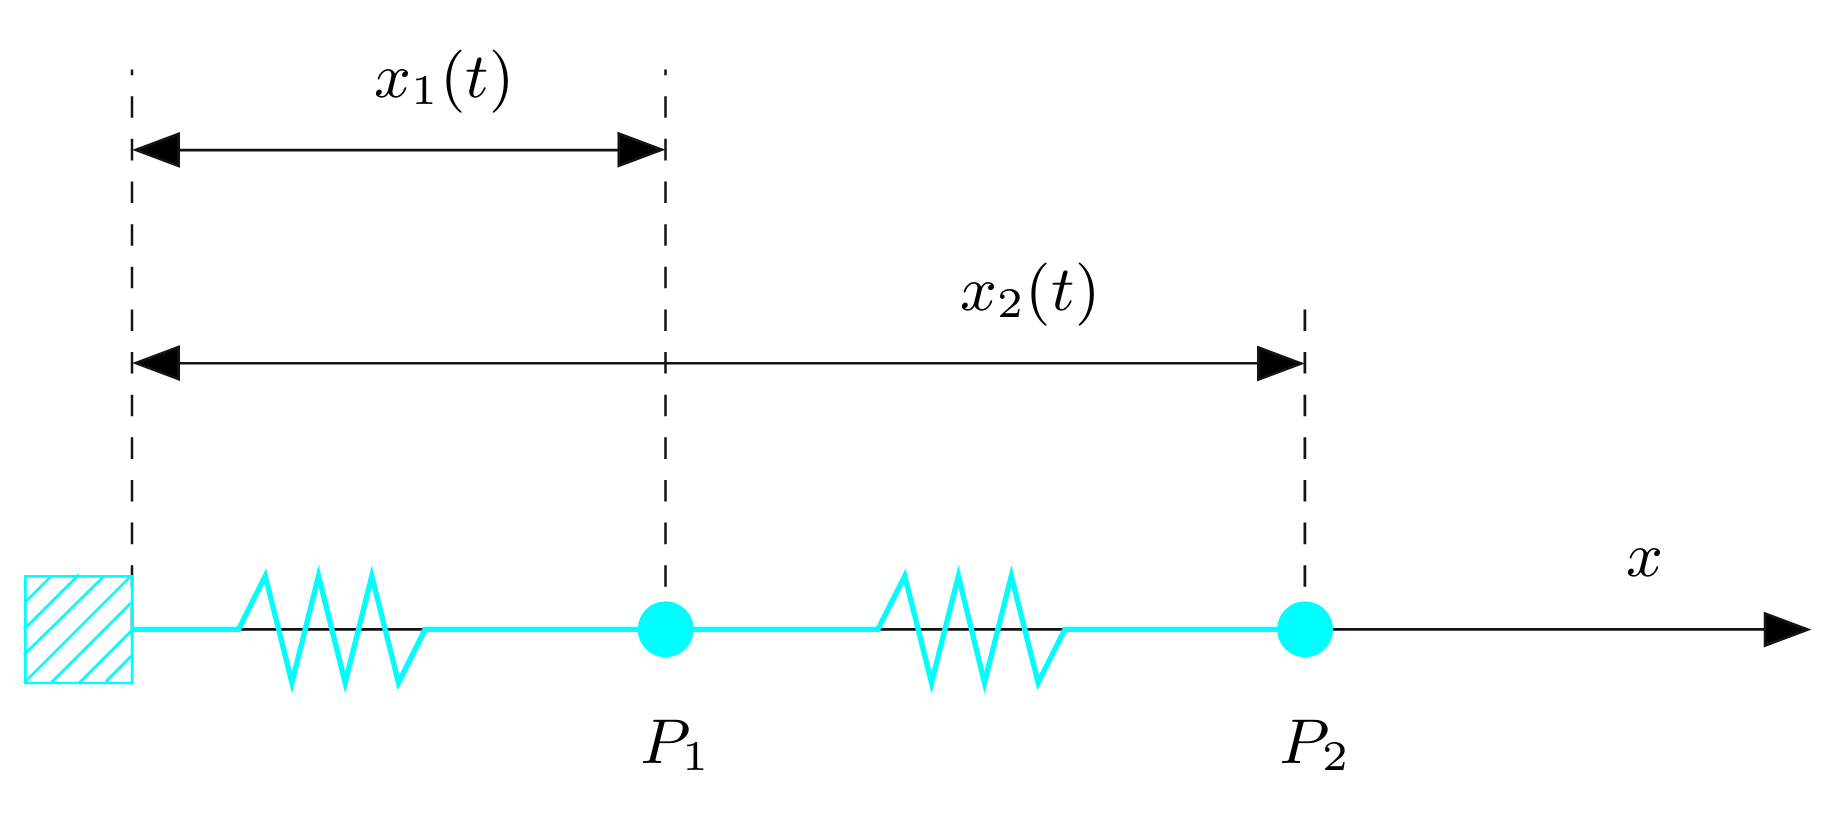
\includegraphics[scale=0.27]{pictures/ressort.png}
	\end{figure}
	Le principe fondamentale de la dynamique donne
	$$
	m \ddot{x}_1=K\left(x_2-x_1\right)-K x_1, \quad m \ddot{x}_2=K\left(x_1-x_2\right)
	$$
	où $K$ est le coefficient de raideur des deux ressorts.
\end{frame}
\begin{frame}{Motivation : Problème (Ressorts élastiques)}
	On s'intéresse aux oscillations libres $x_i=a_i \sin (\omega t+\phi), i=1,2$, avec $a_i \neq 0$. On trouve dans ce cas
	
	\begin{equation}
		-m a_1 \omega^2=K\left(a_2-a_1\right)-K a_1, \quad-m a_2 \omega^2=K\left(a_1-a_2\right)
		\label{sys63}
	\end{equation}
	
	
	C'est un système $2 \times 2$ homogène qui a une solution non triviale $\mathbf{a}=$ $\left(a_1, a_2\right)^T$ ssi le nombre $\lambda=m \omega^2 / K$ est une valeur propre de la matrice
	$$
	A=\left[\begin{array}{rr}
		2 & -1 \\
		-1 & 1
	\end{array}\right]
	$$
	
	Avec cette définition de $\lambda$, \eqref{sys63} devient $\mathrm{A} \mathbf{a}=\lambda \mathbf{a}$. Comme $p_{\mathrm{A}}(\lambda)=$ $(2-\lambda)(1-\lambda)-1$, les deux valeurs propres sont $\lambda_1 \simeq 2.618$ et $\lambda_2 \simeq 0.382$ et correspondent aux fréquences de vibrations propres $\omega_i=\sqrt{K \lambda_i / m}$ du système.
\end{frame}

\section{Méthodes de type puissance itérée}
\subsection{Puissance itérée}

\begin{frame}{Puissance itérée}
\frametitle{La méthode de la puissance}

On va donner dans cette section la méthode de la puissance qui permet de calculer une approximation de la valeur propre de plus grand module ainsi que celle d’un vecteur propre associé à cette valeur propre.\\

\begin{center}
    \textbf{Algorithme de la méthode de la puissance}.
\end{center}

\begin{equation}
    \begin{cases}
    x^{(0)} & \text{ donné dans } \mathbf{C}^n \text{ de norme } 1 \\ 
    \text{Pour } & k=0,1, \ldots \text{ calculer :} \\ 
    & y^{(k+1)} = Ax^{(k)}, \\ 
    & x^{(k+1)} = \frac{y^{(k+1)}}{\| y^{(k+1)} \|_2}, \\ 
    & \lambda^{(k+1)} = (x^{(k)})^* Ax^{(k)} = (x^{(k)})^* y^{(k+1)}.
    \end{cases}
    \label{eq:1}
\end{equation}

\end{frame}


\begin{frame}{Puissance itérée}
	\begin{theorem}
			Soit $A$ une matrice carrée d'ordre $n$, diagonalisable et de valeurs propres $\lambda_i, 1 \leq i \leq n$, comptées avec leur ordre de multiplicité, et vérifiant :
		
		$$
		0 \leq\left|\lambda_1\right| \leq \cdots \leq\left|\lambda_{n-1}\right|<\left|\lambda_n\right|
		$$
		
		
		Soit $\left(u_i\right)_{1 \leq i \leq n}$ une base normée de vecteurs propres de $A$ associés aux valeurs propres $\lambda_i$. Si $x^{(0)}=\sum_{i=1}^n \alpha_i u_i$ est tel que $\alpha_n \neq 0$, alors la méthode de la puissance converge au sens suivant :
	
        \begin{equation}
        			\lim _{k \rightarrow+\infty} \lambda^{(k)}=\lambda_n 
		    \label{eq:2}
		\end{equation}
        		\begin{equation}
			\lim _{k \rightarrow+\infty}\left(x^{(k)}-\beta^k \gamma u_n\right)=0
		    \label{eq:3}
		\end{equation}

		où $\beta=\frac{\lambda_n}{\left|\lambda_n\right|}$ et $\gamma$ est un nombre complexe de module 1.
		
	\end{theorem}

\end{frame}
\begin{frame}{Puissance itérée}
			Montrons \eqref{eq:3}. Posons pour cela, $z^{(0)}=x^{(0)}$ et $z^{(k)}=A^k x^{(0)}$ pour $k \geq 1$. On a alors
		
		\begin{equation}
		   		x^{(k)}=\frac{y^{(k)}}{\left\|y^{(k)}\right\|_2}=\frac{A x^{(k-1)}}{\left\|A x^{(k-1)}\right\|_2}=\frac{A^k x^{(0)}}{\left\|A^k x^{(0)}\right\|_2}=\frac{z^{(k)}}{\left\|z^{(k)}\right\|_2}
                \label{eq:4}
		\end{equation}

		
		
		
		Dans \eqref{eq:4} la 3-ème égalité peut être démontrée par récurrence sur $k$.
		Par ailleurs, on a
		
		\begin{equation}
		    		\begin{aligned}
			z^{(k)}=A^k x^{(0)} & =\sum_{i=1}^n \alpha_i A^k u_i=\sum_{i=1}^n \alpha_i \lambda_i^k u_i \\
			& =\alpha_n \lambda_n^k u_n+\sum_{i=1}^{n-1} \alpha_i \lambda_i^k u_i
		\end{aligned}
        \label{eq:5}
		\end{equation}

	
		
		
		D'où
		
\begin{equation}
    		\frac{z^{(k)}}{\lambda_n^k}-\alpha_n u_n=\sum_{i=1}^{n-1} \alpha_i\left(\frac{\lambda_i}{\lambda_n}\right)^k u_i
            \label{eq:6}
\end{equation}
		
		
	
\end{frame}
\begin{frame}{Puissance itérée}
	Or, pour tout $i \in\{1,2, \ldots, n-1\}$, on a $\left|\lambda_i\right|<\left|\lambda_n\right|$. Et par suite, on obtient
		
\begin{equation}
    		\lim _{k \rightarrow+\infty} \frac{z^{(k)}}{\lambda_n^k}=\alpha_n u_n
            \label{eq:7}
\end{equation}
		
		et donc
		
\begin{equation}
    		\lim _{k \rightarrow+\infty} \frac{\left\|z^{(k)}\right\|_2}{\left|\lambda_n^k\right|}=\left|\alpha_n\right|\left\|u_n\right\|_2=\left|\alpha_n\right|
            \label{eq:8}
\end{equation}
        		puisque $u_n$ est de norme égale à 1 . Utilisant l'hypothèse $\alpha_n \neq 0$, on obtient, d'après \eqref{eq:7} et \eqref{eq:8} :
		
\begin{equation}
    		\lim _{k \rightarrow+\infty} \frac{z^{(k)}}{\left\|z^{(k)}\right\|_2} \frac{\left|\lambda_n^k\right|}{\lambda_n^k}=\frac{\alpha_n}{\left|\alpha_n\right|} u_n
            \label{eq:9}
\end{equation}
\end{frame}
\begin{frame}{Puissance itérée}
		En posant $\beta=\frac{\lambda_n}{\left|\lambda_n\right|}$ et $\gamma=\frac{\alpha_n}{\left|\alpha_n\right|}$, on obtient, grâce à \eqref{eq:4} et \eqref{eq:8} :
		
		$$
		\lim _{k \rightarrow+\infty}\left(x^{(k)}-\beta^k \gamma u_n\right)=0
		$$
		Ce qui prouve \eqref{eq:3}.
		Prouvons \eqref{eq:2}. Utilisant \eqref{eq:4} et \eqref{eq:5}, on obtient
        
       
		Posons
\begin{align}
	x^{(k)} &= \frac{z^{(k)}}{\|z^{(k)}\|_2} = \frac{1}{\|z^{(k)}\|_2} \lambda_n^k \left( \alpha_n u_n + \sum_{i=1}^{n-1} \alpha_i \left( \frac{\lambda_i}{\lambda_n} \right)^k u_i \right) \label{eq:5.22-first} \\
	&= \frac{\alpha_n \lambda_n^k}{\|z^{(k)}\|_2} u_n + \frac{\lambda_n^k}{\|z^{(k)}\|_2} \sum_{i=1}^{n-1} \alpha_i \left( \frac{\lambda_i}{\lambda_n} \right)^k u_i. \label{eq:5.22-second}
\end{align}		
\begin{equation}
    		\beta_n^k=\frac{\alpha_n \lambda_n^k}{\left\|z^{(k)}\right\|_2} \quad \text { et } \quad \beta_i^k=\beta_n^k \frac{\alpha_i}{\alpha_n}\left(\frac{\lambda_i}{\lambda_n}\right)^k, \text { pour } i \in\{1,2, \ldots, n-1\} .
            \hspace{0cm}\label{eq:11}
\end{equation}

\end{frame}
\begin{frame}{Puissance itérée}
		Utilisant \eqref{eq:9}, on obtient
		
\begin{equation}
    		\lim _{k \rightarrow+\infty}\left|\beta_n^k\right|=1
            \label{eq:12}
\end{equation}
		
		et par suite, d'après \eqref{eq:11}, on a
		
\begin{equation}
    		\lim _{k \rightarrow+\infty}\left|\beta_i^k\right|=0, \quad 1 \leq i \leq n-1
            \label{eq:13}
\end{equation}
		
		puisque $\left|\lambda_i\right|<\left|\lambda_n\right|$ pour tout $i \in\{1,2, \ldots, n-1\}$.
		Par ailleurs, on a, d'après \eqref{eq:5.22-second} et \eqref{eq:11}
		
		$$
		A x^{(k)}=\sum_{i=1}^n \beta_i^k A u_i=\sum_{i=1}^n \beta_i^k \lambda_i u_i
		$$
		
		et
		
		$$
		\left(x^{(k)}\right)^*=\sum_{j=1}^n \bar{\beta}_j^k u_j^*
		$$
		
	
\end{frame}
\begin{frame}{Puissance itérée}
	
		Il s'en suit, grâce à \eqref{eq:1}, que
		
		$$
		\lambda^{(k+1)} \equiv\left(x^{(k)}\right)^* A x^{(k)}=\sum_{i, j=1}^n \beta_i^k \bar{\beta}_j^k \lambda_i u_j^* u_i
		$$
        		
		D'où
		
\begin{equation}
    \lambda^{(k+1)}=\left|\beta_n^k\right|^2 \lambda_n \underbrace{\left\|u_n\right\|_2^2}_{=1}+\sum_{\substack{i, j=1 \\(i, j) \neq(n, n)}}^n \beta_i^k \bar{\beta}_j^k \lambda_i u_j^* u_i
    \label{eq:14}
\end{equation}
		
		
		En passant à la limite lorsque $k \rightarrow+\infty$, on obtient, grâce à \eqref{eq:12} et \eqref{eq:13}
		
		$$
		\lim _{k \rightarrow+\infty} \lambda^{(k)}=\lambda_n
		$$
		
		
		Ce qui prouve \eqref{eq:2} et achève la démonstration.
		
\end{frame}
\begin{frame}{Puissance itérée}
    \( \boldsymbol{Exemple} \).\\
  Soit la matrice \( A = \begin{bmatrix} 2 & -12 \\ 1 & -5 \end{bmatrix} \), avec le vecteur propre \( \mathbf{v} = \begin{bmatrix} 3 \\ 1 \end{bmatrix} \) et la valeur propre \( \lambda = -2 \).
    

  
\end{frame}
\begin{frame}[fragile]{Code Example}
		\begin{lstlisting}
A = [2 -12;
1 -5];
X = [1; 1];
v = 1;

for i = 1:10
fprintf('Iteration %d:\n', i);

% Compute new eigenvector approximation
X = (A * X) / norm(A * X, 2);

% Display eigenvector
disp('Le vecteur propre:');
disp(X);

% Compute eigenvalue approximation
v = X' * A * X;

% Display eigenvalue
fprintf('La valeur propre: %.4f\n\n', v);
end

	
\end{lstlisting}
	
\end{frame}

\begin{frame}{Résultats des Itérations}
    \begin{columns}[T] % Start two columns
        % Left column: Iterations 1 to 5
        \begin{column}{0.5\textwidth}
            \scriptsize
            
            \begin{tabular}{|c|c|c|}
                \hline
                \multirow{2}{*}{Itération} & \multirow{2}{*}{Vecteur propre} & Valeur propre \\
                 & &  \\
                \hline
                1 & $\begin{pmatrix} -0.9285 \\ -0.3714 \end{pmatrix}$ & -2.7586 \\
                2 & $\begin{pmatrix} 0.9417 \\ 0.3363 \end{pmatrix}$ & -2.2760 \\
                3 & $\begin{pmatrix} -0.9457 \\ -0.3251 \end{pmatrix}$ & -2.1214 \\
                4 & $\begin{pmatrix} 0.9473 \\ 0.3204 \end{pmatrix}$ & -2.0572 \\
                5 & $\begin{pmatrix} -0.9480 \\ -0.3183 \end{pmatrix}$ & -2.0278 \\
                \hline
            \end{tabular}
        \end{column}

        % Right column: Iterations 6 to 10
        \begin{column}{0.5\textwidth}
            \scriptsize
            
            \begin{tabular}{|c|c|c|}
                \hline
                \multirow{2}{*}{Itération} & \multirow{2}{*}{Vecteur propre} & Valeur propre \\
                 & &  \\
                \hline
                6 & $\begin{pmatrix} 0.9483 \\ 0.3172 \end{pmatrix}$ & -2.0137 \\
                7 & $\begin{pmatrix} -0.9485 \\ -0.3167 \end{pmatrix}$ & -2.0068 \\
                8 & $\begin{pmatrix} 0.9486 \\ 0.3165 \end{pmatrix}$ & -2.0034 \\
                9 & $\begin{pmatrix} -0.9486 \\ -0.3164 \end{pmatrix}$ & -2.0017 \\
                10 & $\begin{pmatrix} 0.9487 \\ 0.3163 \end{pmatrix}$ & -2.0008 \\
                \hline
            \end{tabular}
        \end{column}
    \end{columns}

 
\end{frame}
\subsection{Puissance inverse}
\begin{frame}{Puissance inverse }
C’est la méthode de la puissance appliquée à la matrice $A^{-1}$, qui permet d’obtenir la
valeur propre de plus petit module de A et un vecteur propre qui lui est associé.
\end{frame}
\begin{frame}{Puissance inverse }
\textbf{Recherche de la valeur propre de plus petit module}\\
La valeur propre de plus grand module de $A^{-1}$ est égale à l'inverse de la valeur propre de $A$ de plus petit module, puisque

$$
\max _i \frac{1}{\left|\lambda_i\right|}=\frac{1}{\min _i\left|\lambda_i\right|}
$$


On applique alors la méthode de la puissance à $A^{-1}$, puis on inverse la valeur propre trouvée, pour obtenir la valeur propre de $A$ de plus petit module ainsi qu'un vecteur propre associé. Cela conduit, en partant de l'algorithme de puissance itérée, à l'algorithme suivant :
$$
\begin{cases}x^{(0)} & \text { donné dans } \mathbf{C}^n \text { de norme } 1 \\ \text { Pour } & k=0,1, \ldots \text { calculer } \\ & y^{(k+1)}=A^{-1} x^{(k)} \\ & x^{(k+1)}=\frac{y^{(k+1)}}{\left\|y^{(k+1)}\right\|_2} \\ & \gamma^{(k+1)}=\frac{1}{\left(x^{(k)}\right)^* A^{-1} x^{(k)}}=\frac{1}{\left(x^{(k)}\right)^* y^{(k+1)}}\end{cases}
$$

\end{frame}
\begin{frame}{Puissance inverse }
Dans la pratique, on ne calcule pas $A^{-1}$, mais on résout successivement les systèmes linéaires $A y^{(k+1)}=x^{(k)}$, par exemple en ayant factorisé $A$ une fois pour toute sous la forme du produit de deux matrices triangulaires : $A=L U$ (ou $P A=L U$ lorsque cela est nécessaire).

\begin{center}
    \textbf{Algorithme de la méthode de la puissance inverse}
\end{center}

\begin{equation}
\begin{cases}x^{(0)} & \text { donné dans } \mathbf{C}^n \text { de norme } 1 \\ \text { Pour } & k=0,1, \ldots \text { calculer } \\ & y^{(k+1)} \text { en résolvant le système } A y^{(k+1)}=x^{(k)} \\ & x^{(k+1)}=\frac{y^{(k+1)}}{\left\|y^{(k+1)}\right\|_2} \\ & \gamma^{(k+1)}=\frac{1}{\left(x^{(k)}\right)^* y^{(k+1)}}\end{cases}
\end{equation}

On a le résultat de convergence suivant.
\end{frame}
\begin{frame}{Puissance inverse }
\begin{corollary}
    Soit $A$ une matrice diagonalisable de valeurs propres $\lambda_i, 1 \leq i \leq n$, vérifiant

$$
0<\left|\lambda_1\right|<\left|\lambda_2\right| \leq\left|\lambda_3\right| \leq \cdots \leq\left|\lambda_n\right|
$$


Soit $\left(u_i\right)_{1 \leq i \leq n}$ une base normée de vecteurs propres de $A$ associés aux valeurs propres $\lambda_i$. Si $x^{(0)}=\sum_{i=1}^n \alpha_i u_i$ est tel que $\alpha_1 \neq 0$, alors la méthode de la puissance inverse converge :

$$
\lim _{k \rightarrow+\infty} \gamma^{(k)}=\lambda_1
$$

\end{corollary}

\textbf{Démonstration.}
Il suffit d'appliquer le théorème de puissance itérée à la matrice $A^{-1}$.
\end{frame}

\subsection{Méthode de la puissance inverse avec translation}

\begin{frame}{Puissance inverse avec translation}
    Elle permet d'obtenir la valeur propre la plus proche d'un nombre donné. Soit $\mu$ un nombre donné. Considérons la matrice $(A-\mu I)$ obtenue à partir de $A$ par la "translation $-\mu I$ " (shift en anglais). \\On applique l'algorithme de la méthode de la puissance inverse à la matrice $(A-\mu I)$. Le plus grand module des valeurs propres de $(A-\mu I)^{-1}$ est $\frac{1}{\min _i\left|\lambda_i-\mu\right|}$, où les $\lambda_i$ sont les valeurs propres de $A$.


\end{frame}
\begin{frame}{Puissance inverse avec translation}
    \textbf{Algorithme de la méthode de la puissance inverse avec translation}

$$
\begin{cases}x^{(0)} & \text { donné dans } \mathbf{C}^n \text { de norme } 1 \\ \text { Pour } & k=0,1, \ldots \text { calculer } \\ & y^{(k+1)} \text { en résolvant le système }(A-\mu I) y^{(k+1)}=x^{(k)} \\ & x^{(k+1)}=\frac{y^{(k+1)}}{\left\|y^{(k+1)}\right\|_2} \\ & \tilde{\gamma}^{(k+1)}=\mu+\frac{1}{\left(x^{(k)}\right)^*(A-\mu I)^{-1} x^{(k)}}=\mu+\frac{1}{\left(x^{(k)}\right)^* y^{(k+1)}}\end{cases}
$$
On a le résultat de convergence suivant.
\end{frame}
\begin{frame}{Puissance inverse avec translation}
    \begin{corollary}
        Soit A une matrice diagonalisable de valeurs propres $\lambda_i, 1 \leq i \leq n$. Soit $\left(u_i\right)_{1 \leq i \leq n}$ une base normée de vecteurs propres de $A$ associés aux valeurs propres $\lambda_i$.
Si $\lambda_{i_0}$ est la valeur propre de A la plus proche de $\mu$ avec de plus

$$
\left|\lambda_{i 0}-\mu\right|<\left|\lambda_i-\mu\right|, \quad \text { pour } \lambda_i \in S p(A) \backslash\left\{\lambda_{i 0}\right\}
$$

et si $x^{(0)}=\alpha_{i_0} u_{i 0}+\sum_{\substack{i=1 \\ i \neq i_0}}^n \alpha_i u_i$ est tel que $\alpha_{i_0} \neq 0$, alors la méthode de la puissance inverse avec translation converge :

$$
\lim _{k \rightarrow+\infty} \widetilde{\gamma}^{(k)}=\lambda_{i_0}
$$
    \end{corollary}
    \textbf{Démonstration.}
Il suffit d'appliquer le théorème du puissance itérée à la matrice $(A-\mu I)^{-1}$.
\end{frame}

\subsection{Méthode de la déflation}

\begin{frame}{La méthode de déflation \cite{tonnoir2018}}
	
	Considérons ici une matrice A symétrique et inversible. Elle est diagonalisable dans une base de vecteurs propres (réels)
	$$
	A=U D U^*
	$$
	où les colonnes de la matrice $U$ sont les vecteurs propres $u_j$ associés aux valeurs propres réelles $\lambda_j$.
	Supposons de plus que les valeurs propres sont toutes différentes et t.q.: $0<\left|\lambda_1\right|<\cdots<\left|\lambda_n\right|$.
	
	Comme on a $x=\langle x, u_1\rangle u_1+\cdots+\langle x, 
	u_n\rangle u_n$, si l'on suppose connu l'élément propre $\langle \lambda_n, u_n\rangle$, on a alors:
	$$
	A^k \left( x - \langle x, u_n \rangle u_n \right) = \lambda_{n-1}^k \left( \langle x, u_{n-1} \rangle u_{n-1} + \sum_{i=1}^{n-2} \left( \frac{\lambda_i}{\lambda_{n-1}} \right)^k \langle x, u_i \rangle u_i \right)
	$$
\end{frame}
\begin{frame}{La méthode de déflation}
	
	On déduit donc qu'une façon d'obtenir la \textit{deuxième plus grande} valeur propre en module consiste simplement à appliquer la puissance itérée en partant d'un vecteur
	$$
	x_0=x-\langle x, u_n \rangle u_n
	$$
	i.e. un vecteur orthogonale à l'espace propre $E\left(u_n\right)$.
	
	\textbf{Remarque:}
	C'est équivalent à appliquer la puissance itérée à la matrice
	$$
	A_2=A-\lambda_n u_n u_n^t
	$$
	dont il est facile de vérifier que le spectre est
	$$
	sp\left(A_2\right)=\left\{0, \lambda_1, \cdots, \lambda_{n-1}\right\}
	$$
	
\end{frame}
\begin{frame}
	De manière similaire, pour obtenir la \textit{deuxième plus petite} valeur propre en module, on utilisera la puissance inverse avec comme vecteur initial : 
	$$x_0 = x-\langle x,u_1 \rangle u_1$$ i.e. un vecteur orthogonale à l'espace propre $E(u_1)$. \\  
	\textbf{Remarque :}
	$$Au=\lambda u \Rightarrow  A^{-1}u = \frac{1}{\lambda}u$$
\end{frame}
\begin{frame}{La méthode de déflation}
	\textbf{Algorithme de déflation (p plus grande v.p.) :} \\
	Pour $k=1$ à $p$\\
	\hspace*{0.4cm} Pour $i=1$  à $ k-1$ \\
	\hspace*{1cm} $x_0 \leftarrow x_0 - \langle x_0, u_i\rangle u_i$
	
	$
	\begin{aligned}
		& \hspace{0.5cm} x_0 \leftarrow x_0 / \|x_0\| \\
		& \hspace{0.5cm} y \leftarrow A x_0 \\
		& \hspace{0.5cm} x_1 \leftarrow y / \|y\|
	\end{aligned}
	$ \\
	\hspace*{0.4cm} Tant que $\left|\left|\langle x_0, x_1\rangle \right|-1\right| \geq \varepsilon$\\
	\hspace*{1cm} $x_0 \leftarrow x_1$\\
	\hspace*{1cm} Pour $i=1$ à $k-1$\\
	\hspace*{1.5cm} $x_0 \leftarrow x_0 - \langle x_0, u_i\rangle u_i$\\
	$
	\begin{aligned}
		& \hspace{1cm} x_0 \leftarrow x_0 / \|x_0\| \\
		& \hspace{1cm} y \leftarrow A x_0 \\
		& \hspace{1cm} x_1 \leftarrow y / \|y\| \\
	\end{aligned}
	$
	\\ \hspace*{0.4cm} $\lambda(k) \leftarrow y(1) / x_0(1) \quad u_k \leftarrow x_0$
	\\ Fin Pour
\end{frame}
\begin{frame}
	
	\textbf{Remarques :}
	\begin{itemize}
		\item[$\circ$] Numériquement, la méthode de déflation est instable. 
		Elle ne peut donc être utilisé que pour déterminer 
		quelques valeurs propres (de plus petits ou plus grands 
		modules)
		\item[$\circ$] Lorsque les valeurs propres sont toutes de modules 
		différents, on peut adapter la méthode de déflation à 
		des matrices non symétriques
		\item[$\circ$] Lorsque des valeurs propres sont distinctes mais de 
		même module, la méthode présente des difficultés
	\end{itemize}
	
\end{frame}


\section{Méthode de Jacobi}
\begin{frame}{Méthode de Jacobi \cite{golub2013} \cite{takahashi2013}}
	Cette méthode s'applique aux matrices \textit{symétriques réelles}. Elle permet d'obtenir une approximation de toutes les valeurs propres et tous les vecteurs propres. 
	
	La matrice A étant symétrique, alors elle est diagonalisable. Et par suite, il existe une matrice orthogonale $O$ telle que $O^T AO$ soit diagonale :
	$$O^T AO = diag(\lambda_1, \lambda_2,...\lambda_n),$$
	
	où les nombres $\lambda_i
	, 1 \leq i \leq n,$ sont les valeurs propres de la matrice A, comptées avec
	leur ordre de multiplicité. Rappelons que les vecteurs colonnes de la matrice $O$ forment un
	ensemble orthonormal de vecteurs propres, le i-ème vecteur colonne étant un vecteur propre
	associé à la valeur propre $\lambda_i$.
\end{frame}
\begin{frame}{Méthode de Jacobi}
	Partant de la matrice $A_0 = A$, la méthode de Jacobi consiste à construire une suite $(Q_k)_k$
	de matrices orthogonales, en s’arrangeant pour que la suite de matrices
	$$A_{k+1} = Q^T
	_{k+1}A_kQ_{k+1},$$
	encore symétriques, converge vers une matrice diagonale $D$ ayant les mêmes valeurs propres
	que $A$. Notons au passage que toutes les matrices $A_k$ admettent les mêmes valeurs
	propres qui sont celles de $A$.
	
	Et si l’on pose $$O_k =Q_1Q_2...Q_k,$$
	alors on obtient :
	$$A_k =O^T_kAO_k.$$
\end{frame}
\begin{frame}{Méthode de Jacobi}
	Ceci montre que si, en plus de la convergence de $A_k$ vers une matrice diagonale $D$, la suite de
	matrices orthogonales $(O_k)_k$ converge vers une matrice orthogonale $O$, alors on a $D = O^TAO$,
	et les vecteurs colonnes de $O$ forment une base orthonormée de vecteurs propres de $A$.
	$\checkmark$Le principe de chaque transformation :
	$$ A_k \rightarrow A_{k+1}=Q^T_{k+1}A_kQ_{k+1}$$
	
	est d’annuler un coefficient non diagonal de $A_k$, d'indices $(p_k, q_k)$ avec $p_k < q_k$ tels que $(A_k)_{p_kq_k}$ soit de plus grand module.
	À cause de la symétrie de $A_k$,en fait, on en annule deux. 
\end{frame}
\begin{frame}{Matrice $\Omega$}
	Les matrices $Q_k$ qu'on utilise sont des matrices orthogonales (que nous appelons les rotations de Jacobi) de la forme :
	\begin{equation}
	\Omega = \left( \begin{array}{ccccccc}
	1 & \cdots & 0 & \cdots & 0 & \cdots & 0 \\
	\vdots & \ddots & \vdots & & \vdots & & \vdots \\
	0 & \cdots & \cos \theta & \cdots & \sin \theta & \cdots & 0 \\
	\vdots & & \vdots & \ddots & \vdots & & \vdots \\
	0 & \cdots & -\sin \theta & \cdots & \cos \theta & \cdots & 0 \\
	\vdots & & \vdots & & \vdots & \ddots & \vdots \\
	0 & \cdots & 0 & \cdots & 0 & \cdots & 1
	\end{array} \right)
	\label{eq:rotation_jacobi}
	\end{equation}
	$\Omega_{pp} = \Omega_{qq} = cos~\theta, ~ \Omega_{pq} = -\Omega_{qp} = sin~ \theta,
	\Omega_{ii}=1, $ \\ $ ~ si ~i \neq p ~et~ i \neq q,
	\Omega_{ij} = 0, ~si~ i\neq j, (i, j) \neq (p, q) ~et~ (i, j) \neq (q, p).$\\
	
\end{frame}
\begin{frame}{Méthode de Jacobi}
	
	
	\begin{theoreme}
		\begin{itemize}
			\item[1)]Si la matrice $A = (a_{ij} )_{1\leq i,j\leq n}$ est symtérique et si $B = \Omega^T A\Omega, alors B = (b_{ij} )_{1\leq i,j\leq n}$
			est symétrique ; et on a
			$$\sum_{i, j} b_{i j}^2=\sum_{i, j} a_{i j}^2$$
			\item[2)]Si $a_{p q} \neq 0$, alors il existe un unique $\theta \in \left] -\frac{\pi}{4}, 0 \right[ \cup \left] 0, \frac{\pi}{4} \right[$ tel que $b_{p q} = 0$, et $\theta$ est déterminé par :
			$$\cot 2 \theta=\frac{a_{q q}-a_{p p}}{2 a_{p q}},-\frac{\pi}{4} \leq \theta \leq \frac{\pi}{4}$$
			
			De plus, on a dans ce cas :$$\sum_i b_{i i}^2=\sum_i a_{i i}^2+2 a_{p q}^2$$
		\end{itemize}
		
		
	\end{theoreme}
\end{frame}
\begin{frame}{Méthode de Jacobi}	
	\textbf{Remarque.}
	\begin{itemize}
		\item[i)]La première égalité signifie que la norme de Frobenius définie par :
		$$\|A\|_F^2 = \sum_{i, j} a_{i j}^2$$ est conservée.
		\item[ii)]Si $a_{p q} \neq 0$, la diagonale de $B$ est globalement plus dominante que celle de $A$. Notons que par différence
		$$
		\sum_{i \neq j} b_{i j}^2=\sum_{i \neq j} a_{i j}^2-2 a_{p q}^2.$$
		
		En d'autres termes, la transformation réduit les éléments hors-diagonaux et renforce la diagonale.
	\end{itemize}
	La répétition de ce type d'opérations devrait "creuser" de plus en plus la partie hors diagonale des matrices successives.
	
\end{frame}
\begin{frame}{Méthode de Jacobi}
	Examinons $B=\Omega^T A \Omega$. On a
	$$
	b_{i j}=\sum_{\alpha=1}^N \omega_{\alpha i} \sum_{k=1}^N a_{\alpha k} \omega_{k j}=\sum_{k=1}^N \sum_{\alpha=1}^N \omega_{\alpha i} \omega_{k j} a_{\alpha k}
	$$
	
	Ainsi
	$$
	\left\{\begin{array}{c}
	\text { si } i \neq p, q \text { et } j \neq p, q \quad b_{i j}=a_{i j} \\
	\text { si } i=p \text { et } j \neq p, q \quad b_{p j}=\cos \theta a_{p j}-\sin \theta a_{p j} \\
	\text { si } i=q \text { et } j \neq p \quad b_{q j}=\sin \theta a_{p j}+\cos \theta a_{q j} \\
	\text { pour } i=j=p \quad b_{p p}=\cos ^2 \theta a_{p p}+\sin ^2 \theta a_{q q}-\sin 2 \theta a_{p q} \\
	\text { pour } i=j=q \quad b_{q q}=\sin ^2 \theta a_{p p}+\cos ^2 \theta a_{q q}+\sin 2 \theta a_{p q} \\
	\text { pour } i=p, j=q \quad b_{p q}=\cos 2 \theta a_{p q}+\frac{\sin 2 \theta}{2}\left(a_{p p}-a_{q q}\right) \\
	\text { le reste est obtenu par symétrie. }
	\end{array}\right.
	$$	
	
	
	
\end{frame}
\begin{frame}{Méthode de Jacobi}
	Si $a_{pq} \neq 0$, on choisit $\theta$ pour que $b_{pq} = 0$ : en particulier tel que
	\[
	\cot 2\theta = \frac{a_{qq} - a_{pp}}{2 a_{pq}}, \quad -\frac{\pi}{4} \leq \theta \leq \frac{\pi}{4}.
	\]
	Pour ce choix de $\theta$, pour calculer les autres coefficients $b_{ij}$ de $B$, il n’est en fait pas nécessaire de calculer $\theta$ lui-même ; on a seulement besoin de calculer $\cos \theta$ et $\sin \theta$.
	
	En effet, on remarque que
	\begin{equation}
	\left[\begin{array}{cc}
	b_{pp} & b_{pq} \\
	b_{qp} & b_{qq}
	\end{array}\right]
	=
	\left[\begin{array}{cc}
	\cos \theta & -\sin \theta \\
	\sin \theta & \cos \theta
	\end{array}\right]
	\left[\begin{array}{cc}
	a_{pp} & a_{pq} \\
	a_{qp} & a_{qq}
	\end{array}\right]
	\left[\begin{array}{cc}
	\cos \theta & \sin \theta \\
	-\sin \theta & \cos \theta
	\end{array}\right]
	\label{eq:851}
	\end{equation}
	
	Posons pour simplifier $c = \cos \theta$ et $s = \sin \theta$.
\end{frame}

\begin{frame}{Méthode de Jacobi}
	Dire que nous diagonalisons dans \eqref{eq:851} revient à dire que
	\begin{equation}
	0=b_{p q}=a_{p q}\left(c^2-s^2\right)+\left(a_{p p}-a_{q q}\right) c s
	\label{bpq0}
	\end{equation}
	
	Si $a_{p q}=0$, nous posons simplement $c=1$ et $s=0$. Sinon, définissons
	$$
	\tau=\cot 2\theta =\frac{a_{q q}-a_{p p}}{2 a_{p q}} \quad \text { et } \quad t=s / c
	$$
	On résout l'équation \eqref{bpq0} ainsi équivalente à 
	$$
	t^2+2 \tau t-1=0
	$$
	et on choisit la racine de plus petit module lorsque $\tau \neq 0$. Puisque $t=\tan \theta$ on a $c = \frac{1}{\sqrt{1+t^2}}$ et $s= \frac{t}{\sqrt{1+t^2}}=ct$
	
	
	En fait, si $\tau \neq 0$, on a :
	$
	t=\frac{ signe(\tau)}{|\tau|+ \sqrt{1+\tau^2}}
	$, et si $\tau = 0$ on choisit $t=1$.
\end{frame}

\begin{frame}{Algorithme de la méthode de Jacobi}
	
	\begin{boxV}
		Partant de $A_0=A$, une itération de la méthode de Jacobi consiste à :
		\begin{itemize}
			\item[-] Déterminer $(p_k, q_k)$ vérifiant $
			\left| (A_k)_{p_k q_k} \right| = \max_{1 \leq i < j \leq n} \left| (A_k)_{ij} \right|;
			$
			\item[-] Déterminer la matrice orthogonale $Q_{k+1}$ définie par
			\[
			Q_{k+1} = \Omega,
			\]
			où $\Omega$ est donnée par \eqref{eq:rotation_jacobi} avec $\theta = \theta_k$, $p = p_k$ et $q = q_k$, et où $\theta_k$ est donnée par
			\[
			\cot 2\theta_k = \frac{(A_k)_{q_k q_k} - (A_k)_{p_k p_k}}{2 (A_k)_{p_k q_k}};
			\]
			\item[-] Calculer $A_{k+1} = Q_{k+1}^T A_k Q_{k+1}$
			(Le coefficient $(A_{k+1})_{p_k q_k} = 0$.) 
		\end{itemize}
	\end{boxV}
\end{frame}
\begin{frame}{Résultats de convergence de la méthode de Jacobi }
	Posons $$A_k = D_k + B_k$$
	où $D_k$ est la matrice diagonale formée par les coefficients diagonaux de $A_k$, et $(B_k)_{ij} = (A_k)_{ij}$ si i = j, et $(B_k)_{ii}=0$.
	
	\begin{theoreme}
		La matrice $B_k$ donnée par (5.45), vérifie
		$$\lim \limits_{\substack{k \to \infty}}
		B_k = 0, \quad  dans~ \mathcal{M}_n(\mathbb{R})$$
	\end{theoreme}
	
	\begin{theoreme}
		Soit $\mathcal{S}_n$ l’ensemble des permutations de ${1, 2, . . . , n}.$ Alors, il existe $\sigma \in \mathcal{S}_n$  telle que
		$$\lim \limits_{\substack{k \to \infty}}
		D_k = diag(\lambda_{\sigma(1)}, \lambda_{\sigma(2)},...,\lambda_{\sigma(n)}
		).$$
	\end{theoreme}
	
	
\end{frame}
\begin{frame}{Résultats de convergence de la méthode de Jacobi }
	\begin{theoreme}
		Si toutes les valeurs propres de $A$ sont distinctes, alors la suite de matrices $(O_k)_k$, définies
		par $O_k = Q_1Q_2 ...Q_k, $ est convergente, et la matrice  $O = \lim \limits_{\substack{k \to \infty}}
		O_k$ est orthogonale, et ses
		colonnes sont des vecteurs propres de $A$ associés aux valeurs propres 
		$\lambda_{\sigma(1)}, \lambda_{\sigma(2)},...,\lambda_{\sigma(n)}
		.$
	\end{theoreme}
	\textbf{Remarque.} La détermination de $a_{p q}^k$ comme indiquée dans la méthode classique est relativement coûteuse si la taille de la matrice est importante. On lui préfère souvent les choix suivants :
	\begin{itemize}[label= \ding{228}]
		\item Méthode de Jacobi cyclique : on annule successivement tous les éléments hors diagonaux par un balayage cyclique par exemple ligne par ligne de la gauche jusqu'à la diagonale. Bien sûr, si un élément est nul, on passe au suivant.
		\item Méthode de Jacobi avec seuil : on procède an même balayage, mais on omet d'annuler les éléments inférieurs à un certain seuil qu'on diminue à chaque balayage.
	\end{itemize}
\end{frame}

\section{La méthode de Givens-Householder (bissection)}
\begin{frame}{Introduction \cite{ciarlet2006introduction}}
	C’est une méthode particulièrement bien adaptée à la recherche de valeurs propres sélectionnées d’une matrice \textbf{symétrique}, par exemple toutes les valeurs propres situées dans un intervalle déterminé à l’avance, ou bien les valeurs propres d’un rang donné (en les supposant ordonnées par ordre croissant), etc. Par contre, cette méthode ne permet pas le calcul des vecteurs propres.
	
	La méthode de Givens-Householder (ou bissection) comprend deux étapes:
	
	\textbf{- 1ère étape : tridiagonalisation}
	
	Étant donnée une matrice symétrique \( A \), on détermine une matrice orthogonale \( P \) (d’un type particulier) telle que la matrice (symétrique) \( P^T A P \) soit tridiagonale. Cette étape, qui ne nécessite qu’un nombre fini d’opérations élémentaires, constitue la méthode de Householder de réduction d’une matrice symétrique à la forme tridiagonale.
	
	\textbf{– 2ème étape : bissection}
	
	On est ainsi ramené au calcul des valeurs propres d’une matrice symétrique tridiagonale, qui s’effectue par la méthode de Givens, appelée encore méthode de la bissection. 
\end{frame}
\subsection{Méthode de Householder}
\begin{frame}{Factorisation de Householder}
	\begin{definition}
		\textit{Soit $v \in \mathbb{K}^n \setminus \{0\}$. On appelle matrice de Householder la matrice de la forme :}
		\[
		H(v) = I_n - 2 \frac{v v^*}{v^* v} = I_n - 2 \frac{v v^*}{\|v\|^2}.
		\]
		Par convention, la matrice identité est considérée comme étant une matrice de Householder.
		
	\end{definition}
	\textbf{proposition}
	\textit{Les matrices de Householder sont Hermitiennes et unitaires, de déterminant égal à $-1$.}
	
	
\end{frame}
\begin{frame}{Factorisation de Householder}
	\textbf{Démonstration :} Soit $v \in \mathbb{K}^n \setminus \{0\}$ et $v^\perp$ un vecteur orthogonal à $v$. La matrice $H(v)$ est \textit{hermitienne}. En effet, on a :
	\[
	(H(v))^* = I_n - 2 \frac{(v v^*)^*}{\|v\|^2} = I_n - 2 \frac{v v^*}{\|v\|^2} = H(v).
	\]
	Elle est également \textit{unitaire}, car on a :
	\[
	H(v) (H(v))^* = \left( I_n - 2 \frac{v v^*}{\|v\|^2} \right) \left( I_n - 2 \frac{v v^*}{\|v\|^2} \right).
	\]
	Développons cette expression :
	\[
	= I_n - 4 \frac{v v^*}{\|v\|^2} + 4 \frac{(v v^*)(v v^*)}{\|v\|^4}
	\]
	\[
	= I_n - 4 \frac{v v^*}{\|v\|^2} + 4 \frac{v (v^* v) v^*}{\|v\|^4}.
	\]
	
\end{frame}

\begin{frame}{Factorisation de Householder}
	Or, $v^* v = \|v\|^2$, donc :
	\[
	= I_n - 4 \frac{v v^*}{\|v\|^2} + 4 \frac{v v^*}{\|v\|^2} = I_n.
	\]
	On remarque que $H(v) v^\perp = v^\perp$. Ainsi, $1$ est valeur propre de $H(v)$ de multiplicité $n - 1$. De plus, $H(v) v = -v$. Ainsi, $-1$ est valeur propre de $H(v)$ de multiplicité $1$. Le déterminant d’une matrice étant égal au produit de ses valeurs propres, on obtient bien $\det(H(v)) = -1$.
	
	
\end{frame}
\begin{frame}{Factorisation de Householder}
	\begin{theorem}
		\textit{Soit $v \in \mathbb{K}^n$ tel que $\sum\limits_{i=2}^{n} |v_i| > 0$. Alors on peut construire deux matrices de Householder $H(w_+)$, $H(w_-)$ telles que le vecteur $H(w_\pm)v$ soit colinéaire à $e_1$, le premier vecteur de la base canonique de $\mathbb{K}^n$. Plus précisément, soit $\alpha$ tel que $v_1 = (v_1, e_1) = |v_1| \exp(i\alpha)$, alors pour $w_\pm := v \pm \|v\| \exp(i\alpha) e_1$, on a :}
		\[
		H(w_\pm)v = \mp \|v\| \exp(i\alpha) e_1.
		\]
	\end{theorem}
\end{frame}
\begin{frame}{Factorisation de Householder}
	\textbf{Démonstration :} Par calcul, on a :
	\[
	H(v \pm \|v\| \exp(i\alpha) e_1)v = v - 2 \frac{(v \pm \|v\| \exp(i\alpha) e_1)(v^* \pm \|v\| \exp(-i\alpha) e_1^*)v}{(v^* \pm \|v\| \exp(-i\alpha) e_1^*)(v \pm \|v\| \exp(i\alpha) e_1)},
	\]
	avec :
	\[
	(v \pm \|v\| \exp(i\alpha) e_1)(v^* \pm \|v\| \exp(-i\alpha) e_1^*)v = (v \pm \|v\|)(\|v\|^2 \pm \|v_1\|),
	\]
	\[
	= \|v\|(\|v\| \pm \|v_1\|)(v \pm \|v\| \exp(i\alpha) e_1).
	\]
	et :
	\[
	(v^* \pm \|v\| \exp(-i\alpha) e_1^*)(v \pm \|v\| \exp(i\alpha) e_1) = \|v\|^2 \pm \|v_1\| \pm \|v_1\| + \|v\|^2,
	\]
	\[
	= 2\|v\|(\|v\| \pm \|v_1\|).
	\]
\end{frame}

\begin{frame}{Factorisation de Householder}
	\textbf{Remarque}\\ 
	1. Si $\sum_{i=2}^{n} |v_i| = 0$, on a encore (on rappelle que la matrice unit\'e est une matrice de Householder particuli\`ere) :
	
	\[
	Iv = \|v\|_2 e_1 \quad \text{si} \quad v_1 \geqslant 0,
	\]
	
	\[
	H(v - \|v\|_2 e_1)v = \|v\|_2 e_1 \quad \text{si} \quad v_1 < 0.
	\]
	2.\ \textit{Pour éviter que le dénominateur $2\|v\|(|\|v\| \pm |v_1||)$ associé à $w_\pm$ soit trop petit, on construira $H(w_+)$ plutôt que $H(w_-)$. Pour $\mathbb{K} = \mathbb{R}$, $\exp(i\alpha) = \pm1$, c’est le signe de $v_1$, on construit alors $H(w_+)$ avec :}
	\[
	w_+ = v + \|v\| e_1 \quad \text{si } v_1 \geq 0,
	\]
	\[
	w_+ = v - \|v\| e_1 \quad \text{si } v_1 < 0.
	\]
	Nous allons maintenant procéder à la factorisation de $A$.
	
\end{frame}

\begin{frame}{Méthode de Householder}
	Soit donc $A=\left(a_{i j}\right)_{1 \leq i, j \leq n}$ une matrice symétrique d'ordre $n$, qu'on écrit sous la forme :
	
	$$
	A =
	\left(
	\begin{array}{c|c}
		a_{11} & a_1^t \\  
		\hline 
		a_1 & \begin{array}{c} \quad \\ \widetilde{A}_1 \\ \quad \end{array}
	\end{array}
	\right) { ou}\ a_1 \in \mathbb{R}^{n-1} \text { et } \tilde{A}_1 \in \mathcal{M}_{n-1}(\mathbb{R})
	$$
	
	
	Décrivons la première étape de la méthode de Householder.
	Si $a_1 \neq 0$, alors il existe une matrice de Householder élémentaire $\widetilde{H}_1$ (symétrique et orthogonale) dans $\mathcal{M}_{n-1}(\mathbb{R})$ telle que l'on ait :
	
	$$
	\tilde{H}_1 a_1=\alpha e^{(1)}=(\alpha, 0, \ldots, 0)^t \in \mathbb{R}^{n-1}, \quad \text { où } \alpha \in \mathbb{R}
	$$
	
	Soit $H_1$ la matrice de $\mathcal{M}_n(\mathbb{R})$ définie par :
	
	$$
	H_1 =
	\left(
	\begin{array}{c|c}
		1 & O \\  
		\hline O & \begin{array}{c} \quad \\ \tilde{H}_1 \\ \quad \end{array}
	\end{array}
	\right)
	$$
	
\end{frame}
\begin{frame}{Méthode de Householder}
	On a alors :
	$$
	\begin{aligned}
		& H_1^T A H_1=\left(\begin{array}{c|c}
			1 & O \\
			\hline O & \begin{array}{c} \quad \\ \tilde{H}_1^T=\tilde{H}_1 \\ \quad \end{array}
		\end{array}\right)\left(\begin{array}{c|c}
			a_{11} & a_1^t \\
			\hline a_1 & \begin{array}{c} \quad \\ \tilde{A}_1 \\ \quad \end{array}
		\end{array}\right)\left(\begin{array}{c|c}
			1 & O \\
			\hline O & \begin{array}{c} \quad \\ \tilde{H}_1 \\ \quad \end{array}
		\end{array}\right) \\
		& =\left(\begin{array}{c|c}
			a_{11} & a_1^t \\
			\hline \widetilde{H}_1 a_1 & \begin{array}{c} \quad \\ \widetilde{H}_1 \widetilde{A}_1 \\ \quad \end{array}
		\end{array}\right)\left(
		\begin{array}{c|c}
			1 & O \\  
			\hline O & \begin{array}{c} \quad \\ \tilde{H}_1 \\ \quad \end{array}
		\end{array}
		\right)=\left(\begin{array}{c|c}
			a_{11} & a_1^t \tilde{H}_1=\left(\alpha e^{(1)}\right)^t \\
			\hline
			\alpha \\ 0 \\ \cdot & \begin{array}{c} \quad \\ \widetilde{H}_1 \tilde{A}_1 \widetilde{H}_1 \\ \quad \end{array}  \\ 0   
		\end{array}\right)
	\end{aligned}
	$$
	
\end{frame}
\begin{frame}{Méthode de Householder}
	D'où l'on obtient :
	
	$$
	H_1^T A H_1=H_1 A H_1=\left(\begin{array}{c|c}
		a_{11} & \alpha\ 0 \cdots 0\\
		\hline
		\alpha \\ 0 \\ \cdot & \begin{array}{c} \quad \\ \widetilde{H}_1 \tilde{A}_1 \widetilde{H}_1 \\ \quad \end{array}  \\ 0   
	\end{array}\right)
	$$
	Notons $A_2$ cette matrice : $A_2=H_1 A H_1$. En notant $A_1=A$ et en suivant la même démarche que ci-dessus, on détermine de proche en proche $(n-2)$ matrices symétriques et orthogonales $H_1, H_2, \cdots, H_{n-2}$ de $\mathcal{M}_n(\mathbb{R})$, telles que les matrices symétriques :
	
\end{frame}
\begin{frame}{Méthode de Householder}
	$$
	A_k=H_{k-1}^T A_{k-1} H_{k-1}=\left(H_1 H_2 \cdots H_{k-1}\right)^T A\left(H_1 H_2 \cdots H_{k-1}\right), \quad 2 \leq k \leq n-1
	$$
	
	soient de la forme :
	
	\begin{figure}[h]
		\centering
		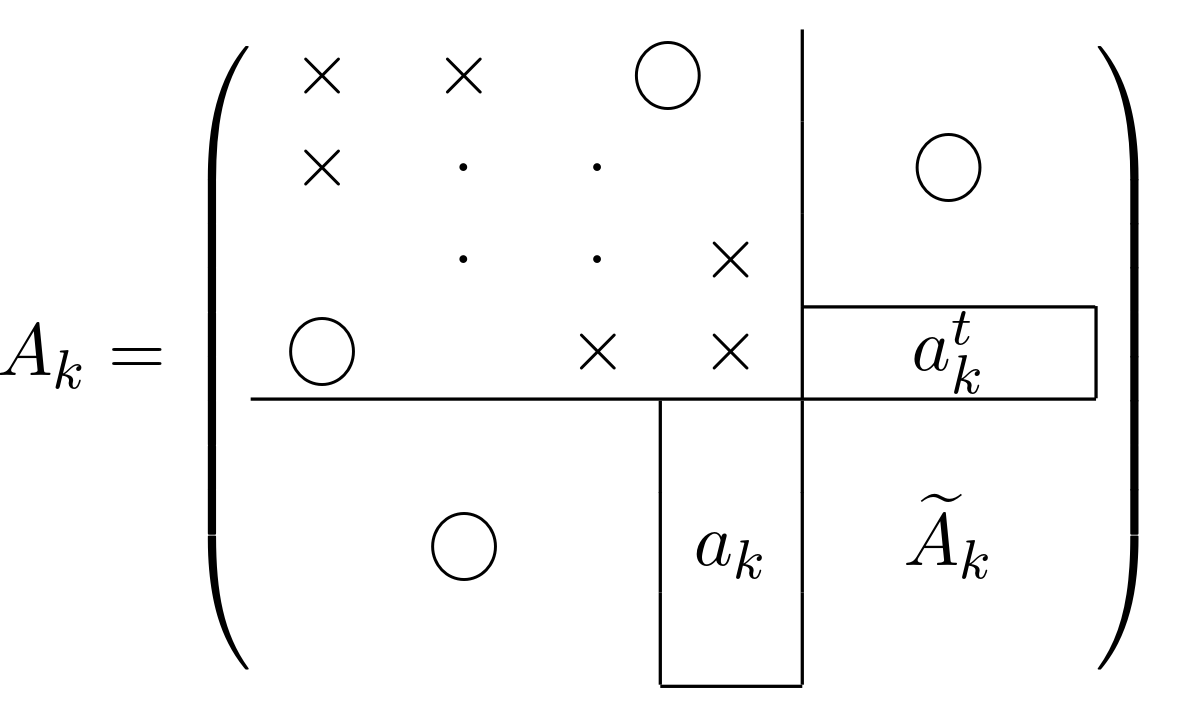
\includegraphics[width=0.5\textwidth]{pictures/one.png}  % Adjust width as needed
		\label{fig:image1}
	\end{figure}
	
	
	
	où $A_k \in \mathcal{M}_{n-k}(\mathbb{R})$, et $a_k$ est le vecteur de $\mathbb{R}^{n-k}$ de composantes les éléments $a_{i k}^k$, $k+1 \leq i \leq n$, de la matrice $A_k=\left(a_{i j}^k\right)_{1 \leq i, j \leq n}$. De la sorte, la matrice
	
	$$
	A_{n-1}=\left(H_1 H_2 \cdots H_{n-2}\right)^T A\left(H_1 H_2 \cdots H_{n-2}\right)
	$$
\end{frame}
\begin{frame}{Méthode de Householder}
	est tridiagonale et est semblable à $A$, puisque la matrice $P=H_1 H_2 \cdots H_{n-2}$ est orthogonale.
	Décrivons à présent la $k$-ème étape de la méthode de Householder qui consiste à tranformer la matrice $A_k$ en la matrice $A_{k+1}=H_k^T A_k H_k$. Chaque transformation $A_k \mapsto A_{k+1}$ est effectuée à l'aide d'une matrice $H_k$ de la forme :
	
	$$
	H_k=\left(\begin{array}{c|c}
		I_k & O \\
		\hline O & \begin{array}{c} \quad \\ \widetilde{H}_k \\ \quad \end{array}
	\end{array}\right)
	$$
	
	où $I_k \in \mathcal{M}_k(\mathbb{R})$ désigne la matrice identité et $\widetilde{H}_k \in \mathcal{M}_{n-k}(\mathbb{R})$ est la matrice de Householder élémentaire vérifiant:
	
	$$
	\widetilde{H}_k a_k=(\alpha, 0, \ldots, 0)^t \in \mathbb{R}^{n-k}, \quad \alpha \in \mathbb{R} .
	$$
\end{frame}
\begin{frame}{Méthode de Householder}
	Si le vecteur $a_k$ est nul, on choisit $\tilde{H}_k=I$, matrice identité de $\mathcal{M}_{n-k}(\mathbb{R})$. Utilisant les propriétés de la multiplication par blocs des matrices, on obtient :
	
	\begin{figure}[h]
		\centering
		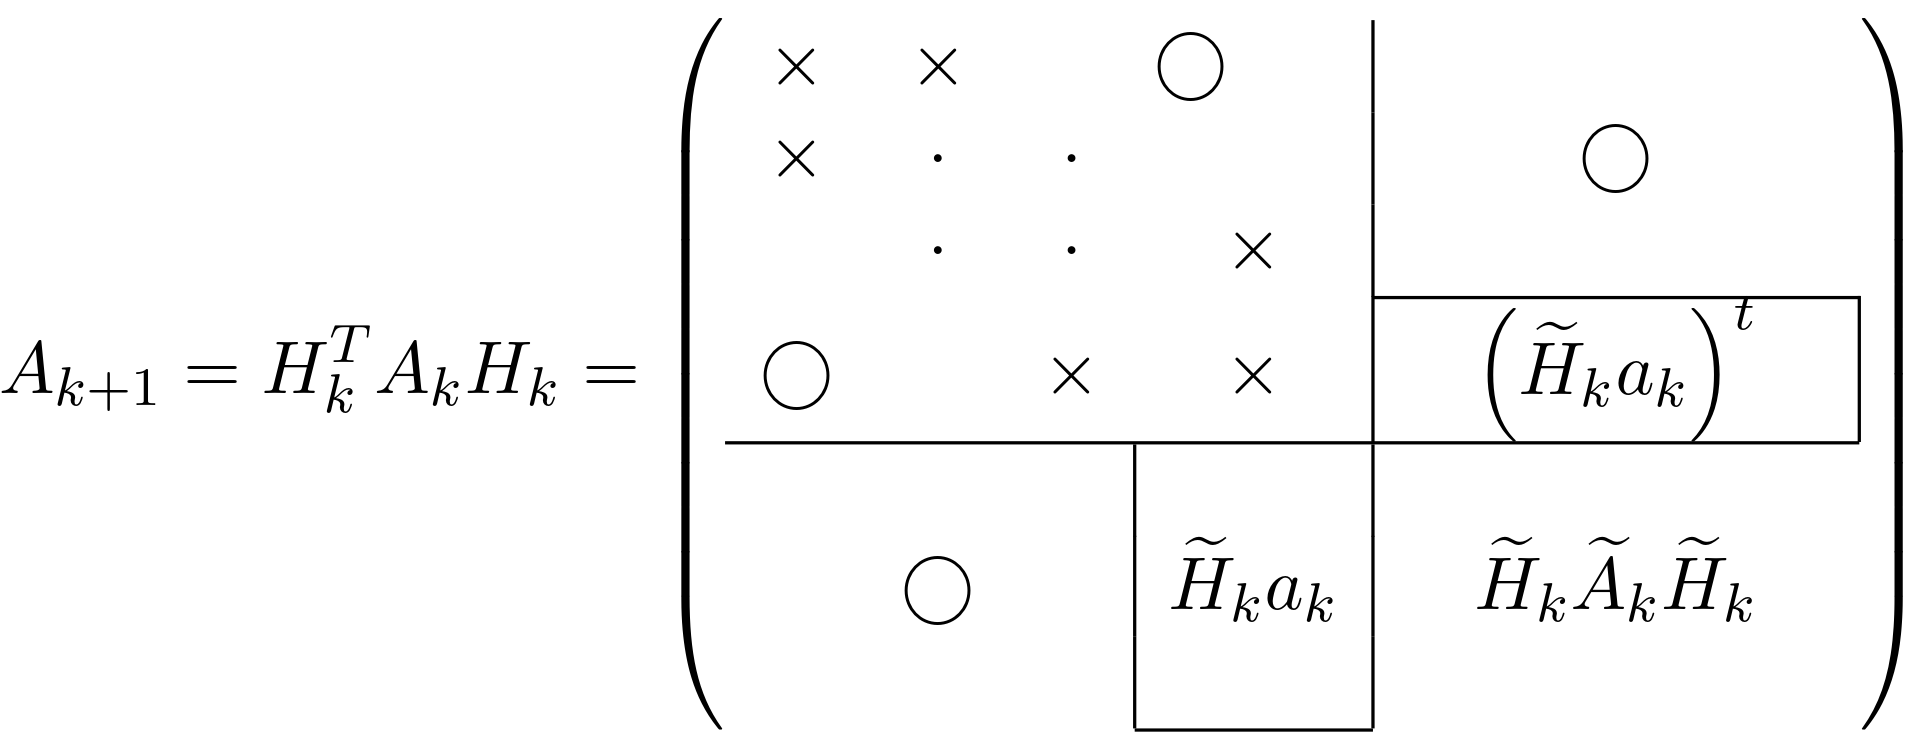
\includegraphics[width=0.8\textwidth]{pictures/two.png}  % Adjust width as needed
		\label{fig:image1}
	\end{figure}
	
\end{frame}
\begin{frame}{Méthode de Householder}
	Plus précisément, on a
	
	\begin{figure}[h]
		\centering
		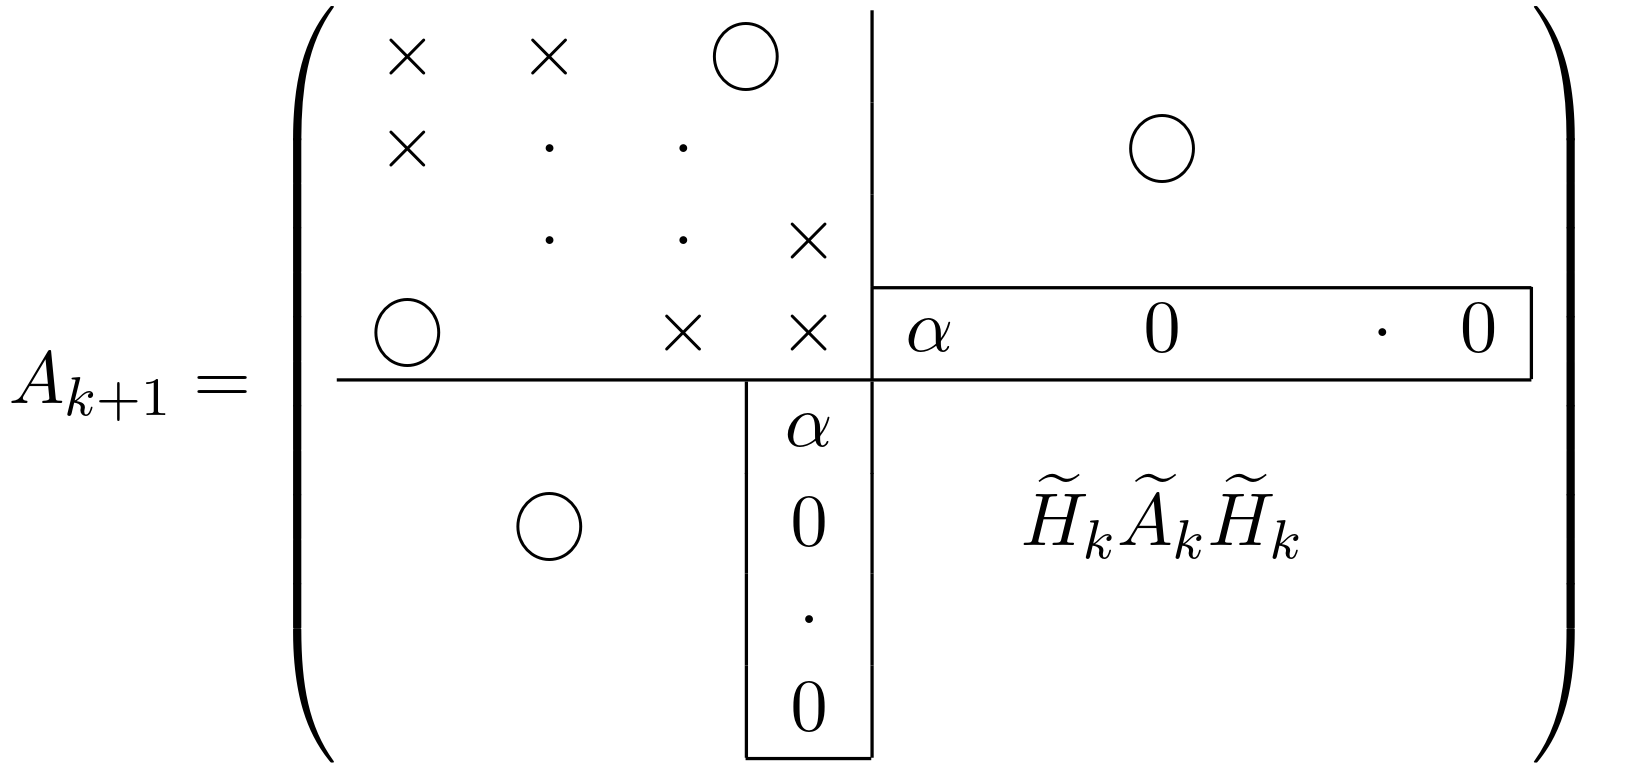
\includegraphics[width=0.65\textwidth]{pictures/three.png}  % Adjust width as needed
		\label{fig:image1}
	\end{figure}
	
	
	avec $a_{i j}^{k+1}=a_{i j}^k$ pour $1 \leq i, j \leq k$.
\end{frame}
\begin{frame}{Méthode de Householder}
	À la fin de la $(n-2)$-ème étape, on obtient une matrice $A_{n-1}$ tridiagonale et semblable à la matrice $A$ :
	
	$$
	A_{n-1}=\left(H_1 H_2 \cdots H_{n-2}\right)^T A\left(H_1 H_2 \cdots H_{n-2}\right)
	$$
	
	
	Récapitulons ce que l'on vient de faire :\\
	\begin{theorem}
		Étant donnée une matrice symétrique $A$ d'ordre $n$, il existe une matrice orthogonale $P$, produit de $(n-2)$ matrices de Householder, telle que la matrice $P^T A P$ soit tridiagonale et semblable à $A$.
	\end{theorem}
	
	
\end{frame}
\subsection{Méthode de Givens}
\begin{frame}{Méthode de Givens}
	Passons ensuite à la description de la \textit{méthode de Givens} de recherche des valeurs propres d’une matrice symétrique tridiagonale :
	
	\[
	B =
	\begin{pmatrix}
		b_1 & c_1 & & & \\
		c_1 & b_2 & c_2 & & \\
		& c_2 & \ddots & \ddots & \\
		& & \ddots & b_{n-1} & c_{n-1} \\
		& & & c_{n-1} & b_n
	\end{pmatrix}.
	\]
	
	
	On observe tout d'abord que si l'un des éléments $c_i$ est nul, la matrice $B$ est déjà décomposée en deux sous-matrices diagonales du même type. On peut donc supposer, sans restreindre la généralité, que
	
	$$
	c_i \neq 0, \quad 1 \leqslant i \leqslant n-1
	$$
	
	
	
	
\end{frame}

\begin{frame}{Méthode de Givens}
	Nous allons commencer par établir que les racines des polynômes caractéristiques des sous-matrices
	$$
	B_i=\begin{pmatrix}
		b_1 & c_1 & & & \\
		c_1 & b_2 & c_2 & & \\
		& c_2 & \ddots & \ddots & \\
		& & \ddots & b_{i-1} & c_{i-1} \\
		& & & c_{i-1} & b_i
	\end{pmatrix}, \quad 1 \leqslant i \leqslant n
	$$
	
	ont des propriétés "d'emboîtement" tout à fait remarquables, illustrées à la figure 6.2-1 ci-après.
\end{frame}

\begin{frame}{Méthode de Givens}
	\begin{theorem}
		Les polynômes $p_i(\lambda), \lambda \in R$, définis pour $i=0,1, \ldots, n$, par les formules de récurrence :
		
		$$
		\begin{aligned}
			p_0(\lambda) & =1 \\
			p_1(\lambda) & =b_1-\lambda \\
			p_i(\lambda) & =\left(b_i-\lambda\right) p_{i-1}(\lambda)-c_{i-1}^2 p_{i-2}(\lambda), \quad 2 \leqslant i \leqslant n
		\end{aligned}
		$$
		
		ont les propriétés suivantes :
		\\\ \ \ \ (1) Le polynôme $p_i$ est le polynôme caractéristique de la matrice $\mathrm{B}_i, 1 \leqslant i \leqslant n$;
		\\\ \ \ \ (2) $\lim _{\lambda \rightarrow-\infty} p_i(\lambda)=+\infty, \quad 1 \leqslant i \leqslant n $;
		\\\ \ \ \ (3) $p_i\left(\lambda_0\right)=0 \Rightarrow p_{i-1}\left(\lambda_0\right) p_{i+1}\left(\lambda_0\right)<0, \quad 1 \leqslant i \leqslant n-1$;
		\\\ \ \ \ (4) Le polynôme $p_i$ possède i racines réelles distinctes, qui séparent les $(i+1)$ racines du polynôme $p_{i+1}, 1 \leqslant i \leqslant n-1$, comme l'indique la figure ci-dessous.
	\end{theorem}
\end{frame}
\begin{frame}{Méthode de Givens}
	\begin{figure}[h]
		\centering
		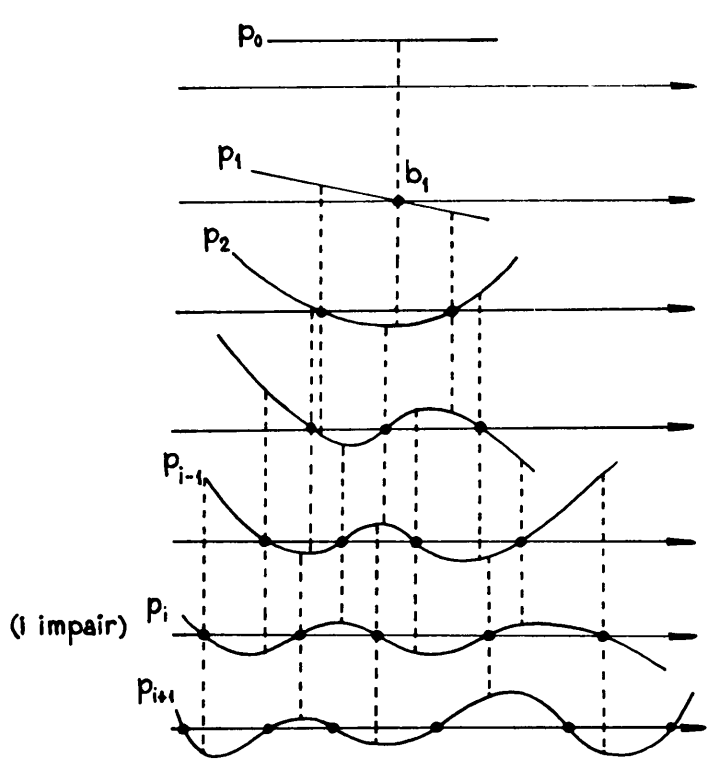
\includegraphics[width=0.65\textwidth]{pictures/four.png}  % Adjust width as needed
		\label{fig:image1}
	\end{figure}
\end{frame}

\begin{frame}{Méthode de Givens}
	\textbf{Démonstration.} (1) Cette propriété se vérifie en développant le déterminant de la matrice \( (B_i - \lambda I) \) par rapport à la dernière ligne (ou colonne).
	
	(2) On voit aisément par récurrence que le monôme de plus haut degré du polynôme \( p_i \) est \( (-1)^i \lambda^i \).
	
	(3) Supposons que \( p_i(\lambda_0) = 0 \) pour un entier vérifiant \( 1 \leq i \leq n-1 \). De la relation de récurrence, on déduit
	
	\[
	p_{i+1}(\lambda_0) = -c_i^2 p_{i-1}(\lambda_0),
	\]
	
	ce qui entraîne (on a supposé \( c_i \neq 0 \)) :
	
	\[
	\left\{
	\begin{array}{l}
		\text{ou bien } p_{i-1}(\lambda_0) p_{i+1}(\lambda_0) < 0, \\
		\text{ou bien } p_{i-1}(\lambda_0) = p_i(\lambda_0) = p_{i+1}(\lambda_0) = 0.
	\end{array}
	\right.
	\]
	
	
\end{frame}
\begin{frame}{Méthode de Givens}
	Dans la seconde éventualité, la relation de récurrence (jointe à nouveau à l’hypothèse \( c_i \neq 0, 1 \leq i \leq n-1 \)) montre que
	
	\[
	p_{i}(\lambda_0) = p_{i-1}(\lambda_0) = \dots = p_1(\lambda_0) = p_0(\lambda_0) = 0,
	\]
	
	ce qui est exclu puisque \( p_0(\lambda) = 1 \).
	
	(4) Cette propriété est une conséquence des propriétés (2) et (3). \(\blacksquare\)
\end{frame}

\begin{frame}{Méthode de Givens}
	
	Une suite de polynômes vérifiant les conditions (2), (3), (4) du théorème précédent est appelée suite de Sturm. La méthode de Givens repose sur une propriété tout à fait remarquable d'une telle suite, qui est de permettre un calcul immédiat du nombre des racines $<\mu, \mu \in \mathcal{M}$ donné, de chacun des polynômes de la suite, comme le montre le résultat ci-dessous.
	
\end{frame}
\begin{frame}{Méthode de Givens}
		\begin{theorem}
		Soit $i$ un entier vérifiant $1 \leqslant i \leqslant n$. Étant donné un nombre $\mu \in \mathcal{M} $, on pose
		
		$$
		\operatorname{sgn} p_i(\mu)=\left\{\begin{array}{llll}
			\text { signe de } & p_i(\mu) & \text { si } & p_i(\mu) \neq 0 \\
			\text { signe de } & p_{i-1}(\mu) & \text { si } & p_i(\mu)=0
		\end{array}\right.
		$$
		
		
		Alors le nombre $N(i ; \mu)$ de changements de signes entre éléments consécutifs de l'ensemble ordonné
		
		$$
		E(i ; \mu)=\left\{+, \operatorname{sgn} p_1(\mu), \operatorname{sgn} p_2(\mu), \ldots, \operatorname{sgn} p_l(\mu)\right\}
		$$
		
		est égal au nombre de racines du polynôme $p_i$ qui sont $<\mu$.
	\end{theorem}
		\textbf{Démonstration.} voir \textit{Introduction à l'analyse numérique matricielle et à l'optimisation de Philippe G. Ciarlet, page 122}.
\end{frame}



\begin{frame}{Méthode de Givens}
	\textbf{Remarque.} \\Appelons $M(i ; \mu)$ le nombre de paires consécutives de même signe $(\{+,+\}$ ou $\{-,-\})$ trouvées dans l'ensemble ordonné $E(i ; \mu)$; par exemple, si
	
	$$
	E(10 ; \mu)=\{+,+,-,+,-,-,+,-,-,-,+\}
	$$
	
	$M(10 ; \mu)=4$, tandis que $N(10 ; \mu)=6$. On vérifie d'ailleurs facilement que
	
	$$
	M(i ; \mu)+N(i ; \mu)=i, \quad \text { pour } \quad i=1, \ldots, n
	$$
	
	de sorte que le nombre $M(i ; \mu)$ est égal au nombre de racines du polynôme $p_i$ qui sont $\geqslant \mu$.
\end{frame}
\begin{frame}{Méthode de Givens}
	Le résultat du théorème précédent permet d'approcher d'aussi près qu'on veut les valeurs propres de la matrice $B=B_n$, et même de calculer directement une valeur propre de rang donné. Supposons en effet qu'on souhaite approcher la $i$-ème valeur propre $\lambda_i=\lambda_i^n$ de la matrice $B$, l'entier $i$ étant fixé (on suppose comme précédemment les valeurs propres $\lambda_1, \ldots, \lambda_n$ rangées par ordre croissant; on rappelle qu'elles sont toutes distinctes d'après le théorème de givens.
\end{frame}
\begin{frame}{Méthode de Givens}
\textbf{Application :} \\
On souhaite calculer la valeur propre de \( B \) de rang \( j_0 \) :

\[
\lambda_1 < \lambda_2 < \cdots < \lambda_{j_0} < \cdots < \lambda_n.
\]

On part d’un intervalle \( [\alpha_0, \beta_0] \) qui contient la valeur propre que l’on cherche, par exemple :

\[
[\alpha_0, \beta_0] = [-\|B\|, \|B\|]
\]

où \( \| \cdot \| \) est une norme matricielle. Soit alors :

\[
\mu_0 = \frac{\alpha_0 + \beta_0}{2}.
\]


	
\end{frame}
\begin{frame}{Méthode de Givens}
	Utilisant le théorème précédent, on a : \\
	\begin{itemize}
		\item Si \( N(n, \mu_0) \geq j_0 \), alors \( \lambda_{j_0} \in [\alpha_0, \mu_0] \), \( \beta_1 = \mu_0 \). \\
		\item Si \( N(n, \mu_0) < j_0 \), alors \( \lambda_{j_0} \in [\mu_0, \alpha_0] \), \( \alpha_1 = \mu_0 \).
	\end{itemize}
	
	De telle sorte que \( \lambda_{j_0} \in [\alpha_k, \beta_k] \). \\
	Ainsi, on construit une suite d’intervalles \( [\alpha_k, \beta_k] \) tels que \( \lambda_{j_0} \in [\alpha_k, \beta_k] \). \\
	On arrête alors les itérations lorsque \( |\alpha_k - \beta_k| \leq \varepsilon \), où \( \varepsilon \) est un paramètre assez petit, \\
	et on prend comme approximation de \( \lambda_{j_0} \) la valeur \( (\alpha_k + \beta_k)/2 \).
\end{frame}

\section{Méthode QR}
\begin{frame}{introduction \cite{ciarlet2006introduction}}
	La méthode QR, due à J. C. F. Francis et à V. N. Kublanovskaya, est la méthode la plus couramment utilisée pour le calcul de l’ensemble des valeurs propres d’une \textit{matrice quelconque}, notamment non symétrique. Naturellement, elle s’applique \textit{a fortiori} aux matrices symétriques, pour lesquelles elle est au moins autant efficace que la méthode de Jacobi.
	
	Nous indiquerons ensuite quelques compléments, concernant notamment la mise en œuvre pratique de la méthode.
\end{frame}
\begin{frame}{factorisation QR d’une matrice}
	\begin{theorem}
		Étant donné une matrice \( A \) d’ordre \( n \), il existe une matrice unitaire \( Q \) et une matrice triangulaire supérieure \( R \) telles que  
		
		\[
		A = QR.
		\]
		
		\textit{De plus, on peut s’arranger pour que les éléments diagonaux de la matrice \( R \) soient tous \( \geq 0 \). Si la matrice \( A \) est inversible, la factorisation \( A = QR \) correspondante est alors unique.}
	\end{theorem}
	\textbf{Démonstration.} En général, la démonstration repose sur les matrices générées par Householder voir \textit{Introduction à l'analyse numérique matricielle et à l'optimisation de Philippe G. Ciarlet, page 102}.
\end{frame}

\begin{frame}{Méthode QR}
	Soit donc $A=A_1$ une matrice carrée quelconque ; on écrit sa factorisation $QR$ (théorème 4.5-2), soit $A_1=Q_1 R_1$, puis on forme la matrice $A_2=R_1 Q_1$ ; on écrit la factorisation $QR$ de la matrice $A_2$, soit $A_2=Q_2 R_2$, puis on forme la matrice $A_3=R_2 Q_2$, et ainsi de suite :
	
	\[
	\begin{aligned}
		A_1 &\rightarrow A_2
		\begin{cases}
			\text{Factorisation } QR: A=A_1=Q_1 R_1, \\
			\text{On pose } A_2=R_1 Q_1, \\
			\vdots
		\end{cases}
	\end{aligned}
	\]
	
	\[
	\begin{aligned}
		A_k &\rightarrow A_{k+1}
		\begin{cases}
			\text{Factorisation } QR: A_k=Q_k R_k, \\
			\text{On pose } A_{k+1}=R_k Q_k.\\
			\vdots
		\end{cases}
	\end{aligned}
	\]
	
\end{frame}

\begin{frame}{Méthode QR}
	On obtient ainsi une suite de matrices $A_k$ qui sont toutes semblables à la matrice $A$, puisque  
	
	\[
	\begin{aligned}
		A_2 &= R_1 Q_1 = Q_1^* A Q_1, \\
		& \vdots \\
		A_{k+1} &= R_k Q_k = Q_k^* A_k Q_k = \dots = \left(Q_1 Q_2 \dots Q_k\right)^* A \left(Q_1 Q_2 \dots Q_k\right).
	\end{aligned}
	\]
	
	Sous des hypothèses assez restrictives, nous établissons dans le théorème ci-dessous que les matrices $A_k$ "deviennent" triangulaires supérieures, en ce sens que  
	
	\[
	\lim _{k \rightarrow \infty} (A_k)_{ij} = 0 \quad \text{pour } j<i,
	\]
	tandis que les éléments diagonaux des matrices $\mathrm{A}_k$ convergent vers les valeurs propres de la matrice $A$. 
\end{frame}

\begin{frame}{Méthode QR}
	Mais attention ! On ne peut rien dire de la convergence éventuelle des éléments $(A_k)_{ij}$ pour $i>j$ et donc de la suite $(A_k)$. Cette observation est néanmoins sans importance du point de vue pratique, dans la mesure où l'objectif recherché, c'est-à-dire une approximation des valeurs propres, est effectivement atteint.
	
	
\end{frame}

\begin{frame}{Méthode QR}
	\begin{theorem}
		On suppose que la matrice $A$ est inversible et que ses valeurs propres sont toutes de modules différents. Il existe donc (au moins) une matrice inversible $P$ telle que  
		
		\[
		A = P \Lambda P^{-1}, \quad \text{avec } \Lambda = \operatorname{diag}(\lambda_1, \lambda_2, \dots, \lambda_n),
		\]
		
		et  
		
		\[
		|\lambda_1| > |\lambda_2| > \dots > |\lambda_n| > 0.
		\]
		
		On suppose que la matrice $P^{-1}$ admet une factorisation $LU$ .  
		Alors la suite de matrices $\left(A_k\right)_{k \geqslant 1}$ est telle que  
		
		\[
		\lim _{k \rightarrow \infty} (A_k)_{ii} = \lambda_i, \quad 1 \leqslant i \leqslant n,
		\]
		
		\[
		\lim _{k \rightarrow \infty} (A_k)_{ij} = 0, \quad 1 \leqslant j < i \leqslant n.
		\]
		
	\end{theorem}
	
\end{frame}
\begin{frame}{Méthode QR}
	\textbf{Démonstration.} voir \textit{Introduction à l'analyse numérique matricielle et à l'optimisation de Philippe G. Ciarlet, page 125}.
\end{frame}
\subsection*{Factorisation de Gram-schmidt}

\begin{frame}{construction de QR}
	Indiquons pour terminer une interprétation remarquable de la factorisation QR d’une matrice inversible \( A \). Notant \( a_1, a_2, \dots, a_n \) et \( q_1, q_2, \dots, q_n \) les vecteurs colonnes des matrices \( A \) et \( Q \) respectivement, la relation \( A = QR \) s’écrit aussi  
	
	\[
	\begin{cases}
		a_1 = r_{11} q_1, \\
		a_2 = r_{12} q_1 + r_{22} q_2, \\
		\vdots \\
		a_n = r_{1n} q_1 + r_{2n} q_2 + \dots + r_{nn} q_n,
	\end{cases}
	\]
	
	en désignant par \( r_{ij} \) les éléments de la matrice triangulaire supérieure \( R \). Or, les vecteurs \( q_i \) formant un ensemble orthonormal (c’est une autre façon d’exprimer le caractère unitaire de la matrice \( Q \)), les relations ci-dessus équivalent au \textit{procédé d’orthonormalisation de Gram-Schmidt}. On pouvait d’ailleurs songer à les utiliser pour une construction plus “directe” des matrices \( Q \) et \( R \) .
	
	
\end{frame}
\begin{frame}{Procédé de Gram-Schmidt}
	\textbf{Procédé d'orthonormalisation de Gram-Schmidt}
	
	Pour un espace euclidien, il existe une autre méthode que la méthode de Gauss pour obtenir des bases orthogonales (et par normalisation, des bases orthonormées).
	
	\begin{theorem}
		\textit{Soit \( E \) un espace préhilbertien et soit
			\( \mathcal{U} = (u_i)_{1 \leq i \leq n} \) un système libre de \( E \), où \( 1 \leq n \leq \dim E \). Alors, il existe un et un seul système orthonormé
			\( \mathcal{B} = (e_i)_{1 \leq i \leq n} \) de \( E \) tel que, pour tout $k \in \{1, 2, \dots, n\}$, on ait :}
		
		\[
		\begin{aligned}
			(i) & \quad \text{Vect}(e_1, \cdots, e_k) = \text{Vect}(u_1, \cdots, u_k) \\
			(ii) & \quad \langle e_k, u_k \rangle > 0.
		\end{aligned}
		\]
		
	\end{theorem}
	\textbf{Démonstration.}\textit{Voir le cours du Pr B. Boussouis, Algèbre 5, page 36.}
\end{frame}

\begin{frame}{QR par Gram-Schmidt}
	\textbf{Remarques :}
	

		(1) Dans la pratique, pour orthonormaliser un système libre \( \mathcal{U} = (u_i)_{1 \leq i \leq n} \), on procède comme suit :
		
		\begin{itemize}[label= -]
			\item On calcule d’abord \( \|u_1\| \), puis on pose \( e_1 = \frac{u_1}{\|u_1\|} \).
			\item On calcule ensuite \( v_2 = u_2 - \langle u_2, e_1 \rangle e_1 \), puis on en déduit \( e_2 = \frac{v_2}{\|v_2\|} \).
			\item Une fois construits \( e_1, \dots, e_{k-1} \), on calcule :
			\[
			e_k = \frac{v_k}{\|v_k\|}, \quad \text{où} \quad v_k = u_k - \sum_{j=1}^{k-1} \langle u_k, e_j \rangle e_j, \quad 2 \leq k \leq n.
			\]
		\end{itemize}
		
\end{frame}

\begin{frame}
	\textbf{Remarques :}
	
	
	(2) On a :
		\[
		\forall k \in  1, n , \quad u_k = \sum_{j=1}^{k} \langle u_k, e_j \rangle e_j.
		\]
		
		Donc si \( \mathcal{U} = (u_i)_{1 \leq i \leq n} \) est une base de \( E \), alors \( \mathcal{B} = (e_i)_{1 \leq i \leq n} \) est une base orthonormée (b.o.n) de \( E \).
		
		De plus, la matrice de passage de \( \mathcal{B} \) à \( \mathcal{U} \) est triangulaire supérieure avec des coefficients diagonaux \( \langle u_k, e_k \rangle \) strictement positifs pour \( k = 1, \dots, n \).
	
\end{frame}

\begin{frame}[fragile]{Code - Partie 1}
	\begin{lstlisting}
		% Definition de la matrice A
		A = [1 2 3; 4 5 6; 7 8 0];
		
		% Recuperation des dimensions de la matrice A
		[n, m] = size(A); 
		
		% Initialisation de Q avec A
		Q = A;
		
		% Normalisation de la premiere colonne de Q
		Q(:,1) = Q(:,1) / norm(Q(:,1));
		
		% Processus de Gram-Schmidt pour orthonormaliser les colonnes de Q
		for i = 2:m  % Parcours des colonnes de Q
		for j = 1:i-1  % Projection sur les vecteurs deja orthonormes
		Q(:,i) = Q(:,i) - (A(:,i)' * Q(:,j)) * Q(:,j);
		end
		% Normalisation de la colonne i
		Q(:,i) = Q(:,i) / norm(Q(:,i));
		end
	\end{lstlisting}
\end{frame}

\begin{frame}[fragile]{Code - Partie 2}
	\begin{lstlisting}
		% Initialisation de la matrice triangulaire superieure R
		R = zeros(m, m);
		
		% Calcul des coefficients de R
		for j = 1:m
		for i = 1:j
		R(i, j) = Q(:,i)' * A(:,j);
		end
		end
		
		% Affichage des matrices Q et R
		Q ,R ,Q*R ,Q'*Q 
	\end{lstlisting}
	\[
	Q =
	\begin{bmatrix}
		0.1231 & 0.9045 & -0.4082 \\
		0.4924 & 0.3015 & 0.8165 \\
		0.8616 & -0.3015 & -0.4082
	\end{bmatrix}
	\quad
	R =
	\begin{bmatrix}
		8.1240 & 9.6011 & 3.3235 \\
		0 & 0.9045 & 4.5227 \\
		0 & 0 & 3.6742
	\end{bmatrix}
	\]
	
	\[
	QR =
	\begin{bmatrix}
		1.0000 & 2.0000 & 3.0000 \\
		4.0000 & 5.0000 & 6.0000 \\
		7.0000 & 8.0000 & 0.0000
	\end{bmatrix}
	\quad
	Q^TQ =
	\begin{bmatrix}
		1.0000 & -0.0000 & -0.0000 \\
		-0.0000 & 1.0000 & -0.0000 \\
		-0.0000 & -0.0000 & 1.0000
	\end{bmatrix}
	\]
\end{frame}

\begin{frame}{QR gram-schmidt}
	\textbf{Remarque.}\\
	mais cette méthode, pourtant “naturelle”, est à écarter en règle générale, car elle conduit à des propagations parfois désastreuses d’erreurs d’arrondi : on lui préférera donc sans hésiter la méthode basée sur l’utilisation des matrices de Householder.
\end{frame}
\subsection*{QR Householder}

\begin{frame}{QR Householder}
	Pour obtenir une factorisation $QR$ de la matrice $A$ qui soit stable numériquement, on peut utiliser les matrices de Householder.
	
	Notons $A = [x_1 \cdots x_n]$ où $x_k$, $1 \leq k \leq n$, est la $k$-ième colonne de $A$ et posons $A_0 = A$.
	
	Pour $1 \leq k \leq n$ on calcule $A_k = H_k A_{k-1}$ où la matrice $H_k$ est construite de façon à annuler les $n - k$ dernières coordonnées de la $k$-ième colonne de $A_{k-1}$.
	On vérifie que $H_k A_{k-1}$ laisse invariant les $k - 1$ premières lignes et colonnes de $A_{k-1}$.
\end{frame}


\begin{frame}{QR Householder}
	1. Choisissez \( H_1 \) de manière à ce que  
	\[
	A_1 \equiv H_1 A =
	\begin{bmatrix}
		x & x & x & x \\
		0 & x & x & x \\
		0 & x & x & x \\
		0 & x & x & x
	\end{bmatrix}.
	\]
	
	2. Choisissez  
	\[
	H_2 =
	\begin{bmatrix}
		1 & 0 \\
		0 & H'_2
	\end{bmatrix}
	\]
	de manière à ce que  
	\[
	A_2 \equiv H_2 A_1 =
	\begin{bmatrix}
		x & x & x & x \\
		0 & x & x & x \\
		0 & 0 & x & x \\
		0 & 0 & x & x
	\end{bmatrix}.
	\]
	
\end{frame}


\begin{frame}{QR Householder}
	3. Choisissez  
	\[
	H_3 =
	\begin{bmatrix}
		1 & 0 & 0 \\
		0 & 1 & 0\\
		0& 0 & H'_3
	\end{bmatrix}
	\]
	
	de manière à ce que  
	\[
	A_3 \equiv H_3 A_2 =
	\begin{bmatrix}
		x & x & x & x \\
		0 & x & x & x \\
		0 & 0 & x & x \\
		0 & 0 & 0 & x
	\end{bmatrix}.
	\]
	\\
	On obtient donc $H_n \cdots H_1 A = A_n$ où $A_n = R$ est triangulaire supérieure avec des éléments strictement positifs sur la diagonale.
	
	Donc, $A = (H_1 \cdots H_n) A_n = QR$ où $Q = H_1 \cdots H_n$ vérifie $Q^t Q = I_n$.
	
\end{frame}
\begin{frame}[fragile]{Code - Partie 1}
	\begin{lstlisting}
		% Definition de la matrice A
		A = [1 2 3; 4 5 6; 7 8 0];
		% Initialisation de R avec la matrice A
		R = A;
		% Determination des dimensions de la matrice A
		[n,m] = size(A);
		% Initialisation de la matrice identite de taille m (matrice orthogonale Q)
		Q = eye(m);
		% Initialisation de l indice de ligne
		j = 1;
		% Boucle pour effectuer la decomposition de Householder
		for i = 1:m
		% Extraction de la i-eme colonne de R
		a = R(:,i);
		% Selection du sous-vecteur a partir de l element j jusqu a la fin
		v = a(j:end);
		% Construction du vecteur Householder
		if v(1) >= 0
		w = v;
		w(1) = w(1) + norm(w); % Modification du premier element
		
		
	\end{lstlisting}
\end{frame}

\begin{frame}[fragile]{Code - Partie 2}
	\begin{lstlisting}
		else
		w = v;
		w(1) = w(1) - norm(w); % Modification du premier element
		end
		% Creation d'une matrice identite de la taille de w
		I = eye(length(w));
		% Calcul de la matrice de transformation de Householder
		M = I - (2 * w * w') / (w' * w);
		% Construction de la matrice de transformation globale H
		H = eye(m);
		H(j:m, j:m) = M;
		% Application de la transformation sur R
		R = H * R;
		% Mise a jour de la matrice orthogonale Q
		Q = Q * H;
		% Incrementation de j pour traiter la sous-matrice suivante
		j = j + 1;
		end
		% Affichage des resultats
		R, Q, Q'*Q, Q*R
	\end{lstlisting}
\end{frame}

\begin{frame}{QR Householder}
	Les résultats sont les suivants :
	\[
	R = \begin{pmatrix}
		-8.1240 & -9.6011 & -3.3235 \\
		0.0000  & 0.9045  & 4.5227 \\
		0.0000  & 0.0000  & 3.6742
	\end{pmatrix}
	\]
	
	\[
	Q = \begin{pmatrix}
		-0.1231 & 0.9045 & -0.4082 \\
		-0.4924 & 0.3015 & 0.8165 \\
		-0.8616 & -0.3015 & -0.4082
	\end{pmatrix}
	\]
	
	\[
	Q'*Q = \begin{pmatrix}
		1.0000 & 0.0000 & 0.0000 \\
		0.0000 & 1.0000 & 0.0000 \\
		0.0000 & 0.0000 & 1.0000
	\end{pmatrix}
	\]
	
	\[
	Q*R = \begin{pmatrix}
		1.0000 & 2.0000 & 3.0000 \\
		4.0000 & 5.0000 & 6.0000 \\
		7.0000 & 8.0000 & 0.0000
	\end{pmatrix}
	\]
	
\end{frame}
\begin{frame}{Méthode QR}
	Après avoir déterminé les matrices \( Q \) et \( R \) de la décomposition, nous revenons à l'algorithme QR initial afin de déterminer une matrice tridiagonale semblable à la matrice \( A \).
\end{frame}

\begin{frame}[fragile]{Méthode QR}
	\begin{lstlisting}
		% Initialisation de la matrice A
		A = [1 2 3; 4 5 6; 7 8 0];
		
		% Boucle pour appliquer l algorithme QR 100 fois
		for i = 1:100
		% Decomposition QR de la matrice A
		[Q,R] = qr(A);
		
		% Mise a jour de A avec le produit R*Q
		A = R*Q;
		end
		
		% Affichage de la matrice resultante A
		A
		
		% Calcul et affichage des valeurs propres de la matrice originale
		V = eig(A)
		
	\end{lstlisting}
	
\end{frame}




\begin{frame}{Méthode QR}
	Les résultats sont les suivants :
	\[
	A = \begin{pmatrix}
		12.1229 & -3.7399 & 3.0183 \\
		0.0000  & -5.7345  & 0.9503 \\
		0.0000  & 0.0000  & -0.3884
	\end{pmatrix}
	\]
	
	\[
	V = \begin{pmatrix}
		12.1229 & \\
		-5.7345 & \\
		-0.3884 &
	\end{pmatrix}
	\]
	
\end{frame}


\begin{frame}{Méthode QR}
	\textbf{Remarque.} (Cours de Takéo Takahashi Ecole des Mines de Nancy p.175)\\
	\textbf{1. Convergence du QR} : \\L'hypothèse technique ($
	|\lambda_1| > |\lambda_2| > \dots > |\lambda_n| > 0.$) n'est pas vraiment essentielle. 
	Si elle n'est pas satisfaite, la méthode QR converge cependant, 
	mais les $\lambda_i$ ne sont plus rangées dans l'ordre décroissant des modules.
	
	
	\textbf{2. Triangularisation par blocs} : Si les valeurs propres ont des modules égaux, la matrice \(A_i\) tend vers une forme triangulaire par blocs, chaque bloc correspondant à un module. Cela est fréquent pour des matrices réelles ayant des valeurs propres complexes conjuguées.
	
	\textbf{3. Structure de Hessenberg} : Si \( A \) est sous forme de Hessenberg ou une matrice bande hermitienne, alors les matrices \( A_i \) conservent cette structure. D’où l’intérêt de réduire une matrice à la forme de Hessenberg (ou tridiagonale si elle est hermitienne) avant d'appliquer QR, pour réduire le coût de calcul.
	
\end{frame}

\begin{frame}{Méthode QR}
	\textbf{4. Vecteurs propres et QR} : L’algorithme QR permet aussi le plus souvent l’obtention des vecteurs propres. Il est difficile de donner des énoncés suffisamment généraux, mais on peut s’en convaincre à l’aide du raisonnement approximatif suivant. Notons 
	\[
	\Omega_k = Q_1Q_2...Q_k.
	\]
	On a alors :
	\[
	A_k = \Omega_k^{-1} A \Omega_k.
	\]
	
	Supposons que pour \( k \) grand, \( A_k = T \) soit exactement triangulaire. Alors :
	\[
	A\Omega_k = \Omega_k T
	\]
	
	
	
\end{frame}


\begin{frame}{Méthode QR}
	En particulier :
	\[
	A\Omega_k e_1 = \Omega_k T e_1 = \lambda_1 \Omega_k e_1
	\]
	et \( \Omega_k e_1 \), c’est-à-dire le premier vecteur colonne de \( \Omega_k \), est vecteur propre de \( A \) pour la valeur propre \( \lambda_1 \). Ensuite, on vérifie que pour \( i \geq 2 \), le vecteur \( q^i = (q^i_j)_{j=1, ..., N} \) est vecteur propre pour \( \lambda_i \) s’il vérifie :
	\[
	\begin{cases}
		q^i_j = 0 \quad \forall j = i + 1, ..., N \\
		q^i_i = 1 \\
		q^i_j = - (t_{j,j+1} q^i_{j+1} + ... + t_{ji} q^i_i) / (\lambda_j - \lambda_i) \quad \forall j = i - 1, ..., 1.
	\end{cases}
	\]
	
	Si on ne s’intéresse qu’à quelques vecteurs propres, on peut aussi utiliser la méthode de la puissance itérée avec translation une fois déterminée la valeur propre.
	
\end{frame}



\begin{frame}{Méthode QR}
	\textbf{5. Cas des matrices réelles} : Si \( A \) est réelle, ses valeurs propres complexes ne permettent pas une convergence vers une matrice triangulaire réelle. Une transformation en arithmétique complexe ou des translations successives de la matrice peuvent être nécessaires.
	
	\textbf{6. QR avec translations} : L'algorithme QR avec translations accélère la convergence, qui est normalement linéaire. On choisit un \( s_k \) bien adapté (généralement une valeur propre de la sous-matrice) pour maximiser la vitesse de convergence.
	
	\textbf{7. Performances} : QR reste moins performant que des méthodes plus sophistiquées comme celles de Jacobi lorsqu'il s'agit d'obtenir simultanément toutes les valeurs propres et vecteurs propres.
	
\end{frame}




\section{Méthode SVD (Décompositon en Valeurs Singulières)}
\begin{frame}{La décomposition en valeurs singulières \cite{perrier2011} \cite{quarteroni2010}}
	\begin{theoreme}[Décomposition en valeurs singulières] Soit $A \in \mathbb{C}^{m \times n}$ (réelle ou complexe). Il existe deux matrices orthogonales $U \in \mathbb{C}^{m \times m}$ et $V \in \mathbb{C}^{n \times n}$ telles que:
		$$
		A=U \Sigma V^{\top} \quad \text { avec } \quad \Sigma=\operatorname{diag} (\sigma_1, \ldots,\sigma_p, 0, \ldots, 0 ) \in \mathbb{R}^{m \times n}.
		$$
		avec $p=\min (m, n)$ et $\sigma_1 \geq \ldots \geq \sigma_p \geq 0$.
		Les $\sigma_i$ sont les valeurs singulières de A .
		
		Les matrices sont obtenues comme suit :
		\begin{itemize}
			\item[(i)] les valeurs singulières $\sigma_i$ sont les racines carrées des valeurs propres $\lambda_i$ à la fois de $A^T A$ et $A A^T$ : \[\sigma_i = \sqrt{\lambda_i} \]
			\item[(ii)] $U$ est la matrice des vecteurs propres de $A^T A$.
			\item[(iii)] $V$ est la matrice des vecteurs propres de $A A^T$.
		\end{itemize}
	\end{theoreme}
\end{frame}
\begin{frame}{La décomposition en valeurs singulières}
	
	\textbf{Preuve.}
	$A^T A$ est une matrice $n \times n$ symétrique positive, donc elle admet des valeurs propres réelles positives $(\lambda_1, \ldots, \lambda_n)$ et une base orthonormée de vecteurs propres associés $\left(V_1, \ldots, V_n\right)$ : $A^{\top} A V_i=\lambda_i V_i$
	De plus :
	$$
	V_i^{\top} A^{\top} A V_j=\lambda_j V_i^{\top} V_j=\lambda_j \delta_{i j}
	$$
	
	On pose $\sigma_j=\sqrt{ } \lambda_j$ et pour les $\sigma_j>0$ (par ex $j=0, \ldots, r$ ): $U_j=A V_j / \sigma_j$.
	Les ( $U_1, \ldots U_r$ ) forment une famille orthonormée de $R^n$, que l'on prolonge en une base orthonormée de $R^m$. Alors on a :
	$\left(U^T A V\right)_{i, j}=U_i^T A V_j=V_i^T A^T A V_j / \sigma_i=\sigma_i \delta_{i j}$ si $j \leq r$ et vaut 0 si $j>r$
	
	Donc $\quad U^{\top} A V=\Sigma$ soit $A=U \Sigma V^{\top}$
	
\end{frame}
\begin{frame}{SVD : pseudo-inverse}
	
	\textbf{Définition : pseudo-inverse :} Soit $A \in \mathbb{R}^{m \times n}$ une matrice de rang $r$, ainsi que sa décomposition en valeurs singulières $A=U \Sigma V^{\top}$.
	La matrice $A^{\dagger}=V \Sigma^{\dagger} U^T$ est appelée matrice pseudoinverse ou inverse généralisée de $A$, avec :
	$$
	\Sigma^{\dagger}=\operatorname{diag}\left(1 / \sigma_1, \ldots, 1 / \sigma_r, 0, \ldots, 0\right)
	$$
	
	\textbf{Remarques :}
	\begin{itemize}
		\item[-] $A^{\dagger} A=I_r$ (matrice identité de rang $r$ )
		\item[-] Si $r g(A)=n<m$, alors $A^{\dagger}=\left(A^T A\right)^{-1} A^T$
		\item[-] Si $r g(A)=n=m, A^{\dagger}=A^{-1}$
	\end{itemize}
\end{frame}
\begin{frame}{SVD}
	Un système linéaire $A x = b$ avec $A \in \mathbb{R}^{m \times n}$ est dit \textit{sous-déterminé} si \( m < n \) (infinité de solutions), et \textit{sur-déterminé} si \( m > n \) (pas de solution en
	général).
	\\
	Dans de nombreuses applications : imagerie médicale, sismique, métérologie..., le nombre d’observations $b_j$ est rarement égal au nombre d’inconnues $x_i$.
	\\
	On peut toutefois résoudre le système d'équations normales \begin{equation}
	A^T A x = A^T b : \label{normale}
	\end{equation}
	Le système \eqref{normale} est inversible si et seulement si $A$ est de rang
	maximal $n$, et dans ce cas, la solution $x^*$ du problème $Ax=b$.
	existe et est unique.
\end{frame}
\begin{frame}{Utilisation de la SVD dans les équations normales}
	Utilisons la SVD de \( A \), c'est-à-dire, \( A = U \Sigma V^T \), où $\Sigma$ est donnée par :
	\[
	\Sigma = \begin{pmatrix}
	\sigma_1 & 0 & \cdots & 0 \\
	0 & \sigma_2 & \cdots & 0 \\
	\vdots & \vdots & \ddots & \vdots \\
	0 & 0 & \cdots & \sigma_n \\
	0 & 0 & \cdots & 0 \\
	\vdots & \vdots & \ddots & \vdots \\
	0 & 0 & \cdots & 0
	\end{pmatrix}_{m \times n}
	\]
	Substituons dans les équations normales :
	
	\[
	A^T A = (V \Sigma^T U^T)(U \Sigma V^T) = V \Sigma^T \Sigma V^T
	\]
	Car \( U^T U = I \) (puisque \( U \) est orthogonale). De plus :
	
	\[
	A^T b = (V \Sigma^T U^T) b.
	\]
	
\end{frame}
\begin{frame}
	Les équations normales deviennent :
	\[
	V \Sigma^T \Sigma V^T x = V \Sigma^T U^T b
	\]
	Puisque \( V \) est orthogonale (\( V^T V = I \)), on multiplie des deux côtés par \( V^T (\Sigma^T \Sigma)^{-1} V \) :
	
	\[
	\Sigma^T \Sigma x = \Sigma^T U^T b
	\]
	La matrice \( \Sigma^T \Sigma \) est diagonale avec les termes \( \sigma_i^2 \) (les carrés des valeurs singulières). On peut donc résoudre pour \( x \) :
	
	\[
	x = V (\Sigma^T \Sigma)^{-1} \Sigma^T U^T b
	\]
	
	Ainsi, la solution des équations normales devient :
	\[
	x = A^{\dagger} b,
	\]
	où \( A^{\dagger} \) est la pseudo-inverse  de \( A \).
\end{frame}


\begin{frame}
	La compression d'images peut être réalisée via la décomposition en valeurs singulières (SVD) d'une matrice. Une image en niveaux de gris est représentée par une matrice réelle \( A \) de taille \( m \times n \), où \( m \) et \( n \) sont le nombre de pixels horizontaux et verticaux, et chaque élément \( a_{ij} \) correspond à l'intensité de gris du pixel \( (i,j) \). La SVD décompose \( A \) en :
	\[
	A = U \Sigma V^T = \sigma_1 u_1 v_1^T + \sigma_2 u_2 v_2^T + \dots + \sigma_p u_p v_p^T,
	\]
	où \( u_i \) et \( v_i \) sont les vecteurs colonnes de \( U \) et \( V \), et \( \sigma_1 \geq \sigma_2 \geq \dots \geq \sigma_p \) les valeurs singulières. Les plus grandes contiennent les informations principales, tandis que les petites correspondent aux détails fins ou au bruit. En tronquant à \( k \) termes (\( A_k = \sum_{i=1}^k \sigma_i u_i v_i^T \)), on obtient une image compressée avec une perte de qualité minimale. Pour transmettre \( A_k \), on envoie uniquement \( u_i \), \( v_i \), et \( \sigma_i \) pour \( i = 1, \dots, k \), réduisant considérablement la taille des données.
\end{frame}

\begin{frame}{Exemple :}
	
	L'image (Lena) suivante est largement utilisée pour tester les algorithmes de compression. Dans MATLAB, elle est chargée et stockée dans une matrice A $512 \times 512$.
	\begin{figure}[H]
		
\includegraphics[scale=0.3]{pictures/lena.png}
	\end{figure}
	L’image originale est à gauche. Celle au centre, obtenue avec les 20 premières
	valeurs singulières, bien que simplifiée reste reconnaissable. Avec \( k = 60 \), l'image à droite est très proche de l'originale et nécessite le stockage de 61\,500 coefficients (deux matrices de taille \( 512 \times 60 \) et 60 valeurs singulières), au lieu de 262\,144 pour l'image originale.
\end{frame}
\begin{frame}
	Bref, la SVD utilise les valeurs singulières et les matrices 
	$U, V$ dans diverses appliquations, notamment :
	
	\begin{itemize}[label= $\diamond$]
		\item Résoudre des systèmes linéaires via la pseudo-inverse.
		\item Réduire la dimension en conservant les grandes $\sigma_i$
		\item Analyser les propriétés (rang, conditionnement, normes) de la matrice.
		\item Traiter le bruit et résoudre des problèmes complexes.
	\end{itemize}
\end{frame}

\section{Méthode de Lanczos}
\begin{frame}{Espace de Krylov \cite{golub2013} \cite{demmel1997} \cite{stoer2002} \cite{trefethen1997}}
	L’\textbf{espace de Krylov} d'ordre \(m\) associé à une matrice \(A \in \mathbb{R}^{n \times n}\) (ou \(\mathbb{C}^{n \times n}\)) et à un vecteur initial \(b \in \mathbb{R}^n\) est défini par :
	\[
	\mathcal{K}_m(A, b) = \text{span}\{b, Ab, A^2b, \dots, A^{m-1}b\}
	\]
	Autrement dit, c'est l'espace vectoriel engendré par les premiers \(m\) vecteurs obtenus en appliquant successivement la matrice \(A\) au vecteur \(b\).
	
	\textbf{Intuition} :  
	Dans les méthodes numériques (comme GMRES, Arnoldi, Lanczos), on cherche une solution approchée d’un système \(Ax = b\) dans cet espace de dimension beaucoup plus petite que \(n\).
\end{frame}

\begin{frame}{Matrice de Krylov}
	La \textbf{matrice de Krylov} correspond à l’organisation de ces vecteurs en colonnes :
	\[
	K(A, q, m) = [q \quad Aq \quad A^2q \quad \dots \quad A^{m-1}q] \in \mathbb{R}^{n \times m}
	\]
	Chaque colonne est \(A\) appliquée un certain nombre de fois sur \(b\).
	
	\textbf{Remarque importante} :
	\begin{itemize}
		\item Dans la pratique, pour éviter des bases numériquement instables, on orthonormalise ces vecteurs (ex: via l'algorithme d'Arnoldi pour matrices générales ou de Lanczos pour matrices symétriques).
	\end{itemize}
\end{frame}
\begin{frame}{Méthode de Lanczos}
	Pour générer une base orthonormale d’un sous-espace de Krylov, nous exploitons la connexion entre la tridiagonalisation de \( A \) et la factorisation QR de \( K(A, q_1, n) \).
	
	Rappelons que si \( Q^T A Q = T \) est tridiagonale et \( QQ^T = I_n \), alors
	\[
	K(A, q_1, n) = QQ^T K(A, q_1, n) = Q \left[ e_1 \,|\, Te_1 \,|\, T^2 e_1 \,|\, \cdots \,|\, T^{n-1}e_1 \right]
	\]
	est la factorisation QR de \( K(A, q_1, n) \), où \( e_1 \) et \( q_1 \) sont respectivement les premières colonnes de \( I_n \) et \( Q \). Ainsi, les colonnes de \( Q \) peuvent être générées en tridiagonalisant \( A \) avec une matrice orthogonale dont la première colonne est \( q_1 \).
	
\end{frame}
\begin{frame}{Méthode de Lanczos}
	La tridiagonalisation par transformations de Householder, peut être adaptée à cet objectif. Cependant, cette approche est peu pratique si \( A \) est grande et creuse, car les mises à jour de Householder détruisent presque toujours la structure creuse. En conséquence, des matrices denses de grande taille apparaissent pendant la réduction. Cela suggère de chercher à calculer directement les éléments de la matrice tridiagonale \( T = Q^T A Q \).
	
\end{frame}
\begin{frame}{Méthode de Lanczos}
	Pour cela, désignons les colonnes de \( Q \) par
	\[
	Q = [q_1 \,|\, \cdots \,|\, q_n]
	\]
	et les composantes de \( T \) par
	\[
	T = 
	\begin{pmatrix}
		\alpha_1 & \beta_1 & & & 0 \\
		\beta_1 & \alpha_2 & \beta_2 & & \\
		& \beta_2 & \ddots & \ddots & \\
		& & \ddots & \alpha_{n-1} & \beta_{n-1} \\
		0 & & & \beta_{n-1} & \alpha_n
	\end{pmatrix}.
	\]
	
	En identifiant les colonnes dans \( AQ = QT \), nous concluons que
	\[
	Aq_k = \beta_{k-1}q_{k-1} + \alpha_k q_k + \beta_k q_{k+1},
	\quad (\beta_0 q_0 \equiv 0),
	\] 
\end{frame}
\begin{frame}{Méthode de Lanczos}
	pour \( k = 1 : n-1 \).
	
	L'orthonormalité des vecteurs \( q \) implique
	\[
	\alpha_k = q_k^T A q_k.
	\]
	
	(Une autre manière de voir cela est que \( T_{ij} = q_i^T A q_j \)).
	
	De plus, si nous définissons le vecteur \( r_k \) par
	\[
	r_k = (A - \alpha_k I)q_k - \beta_{k-1}q_{k-1}
	\]
	et s’il est non nul, alors
	\[
	q_{k+1} = \frac{r_k}{\beta_k}
	\]
	où
	\[
	\beta_k = \pm \|r_k\|_2.
	\]
	
	
\end{frame}
\begin{frame}{Méthode de Lanczos}
	Si \( r_k = 0 \), alors l’itération s’interrompt, mais (comme nous le verrons) non sans avoir acquis des informations précieuses sur les sous-espaces invariants.
	
	En ordonnant correctement les formules ci-dessus et en supposant que \( q_1 \in \mathbb{R}^n \) est un vecteur unitaire donné, nous obtenons ce qui peut être considéré comme la « version 0 » de \textit{l'itération de Lanczos}.
\end{frame}
\begin{frame}{Algorithme (Tridiagonalisation de Lanczos)}
	Étant donné une matrice symétrique \( A \in \mathbb{R}^{n \times n} \) et un vecteur unitaire \( q_1 \in \mathbb{R}^n \), l'algorithme suivant calcule une matrice \( Q_k = [q_1 \,|\, \cdots \,|\, q_k] \) à colonnes orthonormées et une matrice tridiagonale \( T_k \in \mathbb{R}^{k \times k} \) telle que \( AQ_k = Q_k T_k \). Les entrées diagonales et superdiagonales de \( T_k \) sont respectivement \( \alpha_1, \ldots, \alpha_k \) et \( \beta_1, \ldots, \beta_{k-1} \). L'entier \( k \) satisfait \( 1 \leq k \leq n \).
\end{frame}
\begin{frame}{Algorithme (Tridiagonalisation de Lanczos)}
	\begin{algorithm}[H]
		\SetAlgoLined
		$k \gets 0$, $\beta_0 \gets 1$, $q_0 \gets 0$, $r_0 \gets q_1$\;
		\While{$k = 0$ \textbf{ou} $\beta_k \neq 0$}{
			$q_{k+1} \gets r_k / \beta_k$\;
			$k \gets k + 1$\;
			$\alpha_k \gets q_k^\top A q_k$\;
			$r_k \gets (A - \alpha_k I)q_k - \beta_{k-1}q_{k-1}$\;
			$\beta_k \gets \|r_k\|_2$\;
		}
	\end{algorithm}
	
	Il n'y a pas de perte de généralité à choisir \( \beta_k \) positif. Les vecteurs \( q_k \) sont appelés \textit{vecteurs de Lanczos}. Il est important de noter qu'il existe de meilleures méthodes numériques pour organiser la construction des vecteurs de Lanczos que l'algorithme précedent comme (l'algorithme de Lanczos, voir Matrix Computations, (Golub) p.562).
\end{frame}

\begin{frame}{Algorithme (Tridiagonalisation de Lanczos)}
	L’itération de Lanczos s’arrête avant une tridiagonalisation complète si \( q_1 \) est contenu dans un sous-espace invariant propre. C’est l’une des plusieurs propriétés mathématiques du procédé que nous résumons dans le théorème suivant. 
\end{frame}
\begin{frame}
	\begin{theorem}
		L'itération de Lanczos (\textit{Algorithme}) s'exécute jusqu’à \( k = m \), où
		\[
		m = \text{rang}(K(A, q_1, n)).
		\]
		De plus, pour \( k = 1:m \), nous avons
		\[
		AQ_k = Q_k T_k + r_k e_k^T 
		\]
		où \( Q_k = [q_1 \,|\, \cdots \,|\, q_k] \) a des colonnes orthonormales qui engendrent \( \mathcal{K}(A, q_1, k) \), \( e_k = I_n(:,k) \),
		
		
		et
		\[
		T_k =
		\begin{pmatrix}
			\alpha_1 & \beta_1 & & & 0 \\
			\beta_1 & \alpha_2 & \beta_2 & & \\
			& \beta_2 & \ddots & \ddots & \\
			& & \ddots & \alpha_{k-1} & \beta_{k-1} \\
			0 & & & \beta_{k-1} & \alpha_k
		\end{pmatrix}.
		\]
	\end{theorem}
	\textbf{Démonstration.}Matrix Computations 4 edition p.550 .
\end{frame}
\section{Conlusion}
\begin{frame}{Conlusion}
	Les méthodes de calcul des valeurs propres et vecteurs propres que nous avons explorées illustrent la richesse et la diversité des approches pour résoudre ce problème central de l’algèbre linéaire. Chacune présente des forces et des limites, adaptées à des contextes spécifiques. La méthode de la puissance, simple et efficace, excelle pour trouver la valeur propre dominante, mais reste limitée pour les spectres complets. Les transformations de Givens et Householder, en réduisant les matrices à des formes condensées (tridiagonale ou Hessenberg), préparent le terrain pour des algorithmes comme QR, qui offre une convergence robuste pour les matrices denses, bien que coûteuse en calculs. La méthode de Jacobi, précise pour les matrices symétriques, devient prohibitive pour les grandes tailles, tandis que la SVD, bien que plus générale, est particulièrement puissante pour les matrices non carrées ou mal conditionnées. Enfin, Lanczos se distingue pour les matrices creuses de grande dimension, comme celles rencontrées en analyse numérique avancée, mais peut être sensible aux erreurs d’arrondi.
\end{frame}

\begin{frame}{Conlusion}
	Le choix d’une méthode dépend donc du type de matrice (symétrique, creuse, dense), de la précision requise, des contraintes computationnelles, et du contexte applicatif — qu’il s’agisse de stabilité en systèmes dynamiques, de compression de données, ou d’analyse spectrale en physique. Ces algorithmes, bien établis, continuent d’évoluer avec des optimisations modernes, notamment pour les calculs parallèles et les applications en apprentissage automatique. En somme, l’étude des valeurs propres et vecteurs propres, à travers ces méthodes, révèle non seulement leur profondeur mathématique, mais aussi leur rôle incontournable comme pont entre théorie pure et applications concrètes, invitant à une exploration toujours plus poussée.
\end{frame}

\begin{frame}[allowframebreaks]
	\frametitle{Références}
	\bibliographystyle{plain}
	\bibliography{references}

\end{frame}

\end{document}
